\chapter{Mesh Approximation and Compression}

Sparse approximation have gained great success on the regular domain
of 2D images. However, the topics of approximating or compressing signals defined
over meshes are much less investigated due to the irregularity of
underlying domains. In this chapter, we
takes an initiative to explore the challenging problem of sparse
approximation of discrete 3D shapes for compressive shape representation.

\section{Introduction}

Conventional Fourier analysis decomposes a signal into mutually
independent components with the multiscale and orthogonal Fourier
bases. Compression is achieved by discarding certain number of
high-frequency Fourier coefficients. This scheme has been transplanted
to mesh compression, using the eigenbases of mesh Laplacian, i.e, the
manifold harmonic basis (MHB), as the Fourier
bases~\cite{Karni2000}. The key disadvantage of Fourier
compression is that the Fourier bases are only localized in the
frequency domain yet having global support in the spatial domain, and
thus are not efficient in encoding local signal information. A popular
and powerful solution is to use wavelet bases, which are functions
localized in both location and frequency and can capture local signal
information in a more compact and efficient way.

In this chapter, we propose to use the spectral graph wavelets (SGW),
pioneered by Hammond et al.~\cite{Hammond2011}, for mesh
compression. To the best of our knowledge, we believe that it is the
first attempt to exploit the SGW in sparse representation, with a
unique application in 3D geometric compression. The SGW has many
attractive properties such as spatial localization, being smooth,
multi-scale, and shape-aware, and being flexible and versatile for 3D
shapes of arbitrary topology and complicated geometry, hence is well
suited for encoding shapes with many local details. We employ the SGW
as shape bases to construct redundant dictionary with multiscale
wavelets centered around each vertex, and employ the simultaneous
orthogonal matching pursuit (S-OMP) algorithm to find a sparse coding
of the original shape geometry. The primary contributions of this work
are hinging upon the unique integration of the spectral graph wavelets
(SGW) and sparse representation and its powerful application in 3D
shape compression. To the best extent of our knowledge, our current
work is the first attempt to employ the SGW in the task of 3D mesh compression.

Through our extensive experiments, we wish to demonstrate that our
compression method outperforms the MHB-based Fourier compression in
terms of compression quality at different compression ratio settings.
Since our sparse shape approximation framework is independent of any
data-specific dictionary design, other formulations of bases or
dictionaries, as well as other powerful sparse approximation
algorithms, can all be migrated into our system with very little extra
workload. So we are expecting further computational improvement in
compression performance in the near future.

\section{Spectral Mesh Compression}

Harmonic analysis techniques such as Fourier transform and wavelet
transform are fundamental tools in compressing images,
audio, and video signals. Prominent applications include the
JPEG~\cite{wallace1992jpeg} and JPEG2000~\cite{skodras2001jpeg} image
compression standards, which are based on 2D discrete cosine transform
and discrete wavelet transform, respectively. The key idea of harmonic
compression is to decompose the original signal into a set of harmonic
basis and reduce the representation size by discarding coefficients
that correspond to much less noticeable signal components.

While traditional harmonic analysis oftentimes uses orthogonal basis,
such as the Fourier basis, recent years have witnessed the increasing
popularity of sparse approximation methods, which enable the utility
of redundant or over-complete dictionaries for signal representation.
From the dictionary of elementary signals, a small subset that can
best capture the structure of the input signal is selected, and the
input signal is approximated by a linear combination of the selected signals.

A 3D mesh can be expressed as the connectivity information of the mesh
topology plus the 3D mesh coordinates. The mesh connectivity defines
the domain of coordinate functions and have several efficient,
lossless coding \cite{Rossignac1999,Gumhold:1998}. To compress the
mesh coordinates, traditional Fourier and wavelet compression
techniques for images can not be directly applied, since 3D meshes
generally do not have a fixed regular graph structure. Consequently,
there is no universally feasible Fourier basis and the dictionary
should be derived from specific object's graph topology.
In~\cite{Karni2000}, Karni and Gotsman employed the mesh
Laplacian eigenbases to encode the mesh geometry, and the compression
is achieved by discarding high-frequency coefficients. Later, Karni
and Gotsman extended the spectral compression method by using fixed
eigenbases derived from a 6-regular mesh to approximate the eigenbases
of the non-regular input meshes, avoiding the cost of Laplacian
decomposition on the decoder side~\cite{karni20013d}.

\section{Mesh Compression via Sparse Approximation}

\subsection{Mesh Laplacian and Manifold Harmonic Basis}
\label{sec:mhb}

Consider a 3D mesh represented as a graph $M=(V,E)$ with vertices $V$
and edges $E$, where $V=\{v_1,v_2,\ldots,v_n\}$. A vector-valued
function $\mathbf{f}:V\to\mathbb{R}^c$ defined on $V$ can be
represented as an $n\times c$ matrix, where the $i$-th row represents
the function value at $v_i$.

The Laplace matrix of mesh $M$ can be defined by the result of applying it to
a function $\mathbf{f}$ defined on $V$:

\begin{equation}
  (L\mathbf{f})_i=\frac{1}{a_i}\sum_{j\in N(i)} w_{ij}(\mathbf{f}_i-\mathbf{f}_j),
\end{equation}

where $N(i)$ denotes the index set of the 1-ring neighbors of $v_i$,
and $a_i$ are the masses associated with each vertex and $w_{ij}$
represents the weight of each edge.

Depending on the choice of $a_i$ and $w_{ij}$, mesh Laplacian may have
many different forms and can be classified as either
\emph{combinatorial} or \emph{geometric}~\cite{Zhang:2010:CGF}. A
combinatorial Laplacian is determined solely by the connectivity of
the mesh. A geometric Laplacian, on the other hand, takes into account
both the topological and geometric information.

Although a geometric Laplacian affords much more precise description
of the mesh geometry, it is not a feasible choice in mesh compression
applications because the geometric information is unknown on the
decoder side. On the other hand, a combinatorial Laplacian can be
easily reconstructed in the decoder size since the mesh connectivity
can be efficiently encoded and transmitted independent of the
geometric coordinates. In this work, we use the graph Laplacian
defined as
\begin{equation}
L_{ij} =
\begin{cases}
1 & \text{if } j \in N(i),\\
-d(i) & \text{if } i=j,\\
0 & \text{otherwise,}
\end{cases}
\end{equation}
where $d(i)$ represents the valence of $v_i$.

The graph Laplacian is symmetric and negative semi-definite, and by
solving the eigenvalue problem $L_s\mathbf{\chi}_k=-\lambda_k\chi_k$
we obtain the eigensystem $\{\lambda_k,\mathbf{\chi}_k\}_{k=0}^{n-1}$,
where $\{\lambda_k,\mathbf{\chi}_k\}$ denotes the $k$-th eigenvalue
and eigenfunction. According to the spectral theorem, the
eigenfunctions $\{\mathbf{\chi}_k\}$ form an complete and orthonormal
basis, called the \emph{Laplacian eigenbasis}, or, in the context of
shape analysis, the manifold harmonic basis
(MHB).  Fig.~\ref{fig:mhb} visualizes the MHB
on an example mesh. It is straightforward to see that the values of
MHB oscillate between negative and positive on the surface, and the
larger the associated eigenvalues, the more frequent the oscillation
becomes, similar to the behaviors of regular Fourier basis functions
in the Euclidean domain.
\begin{figure}
        \centering
        \begin{subfigure}[b]{0.3\linewidth}
                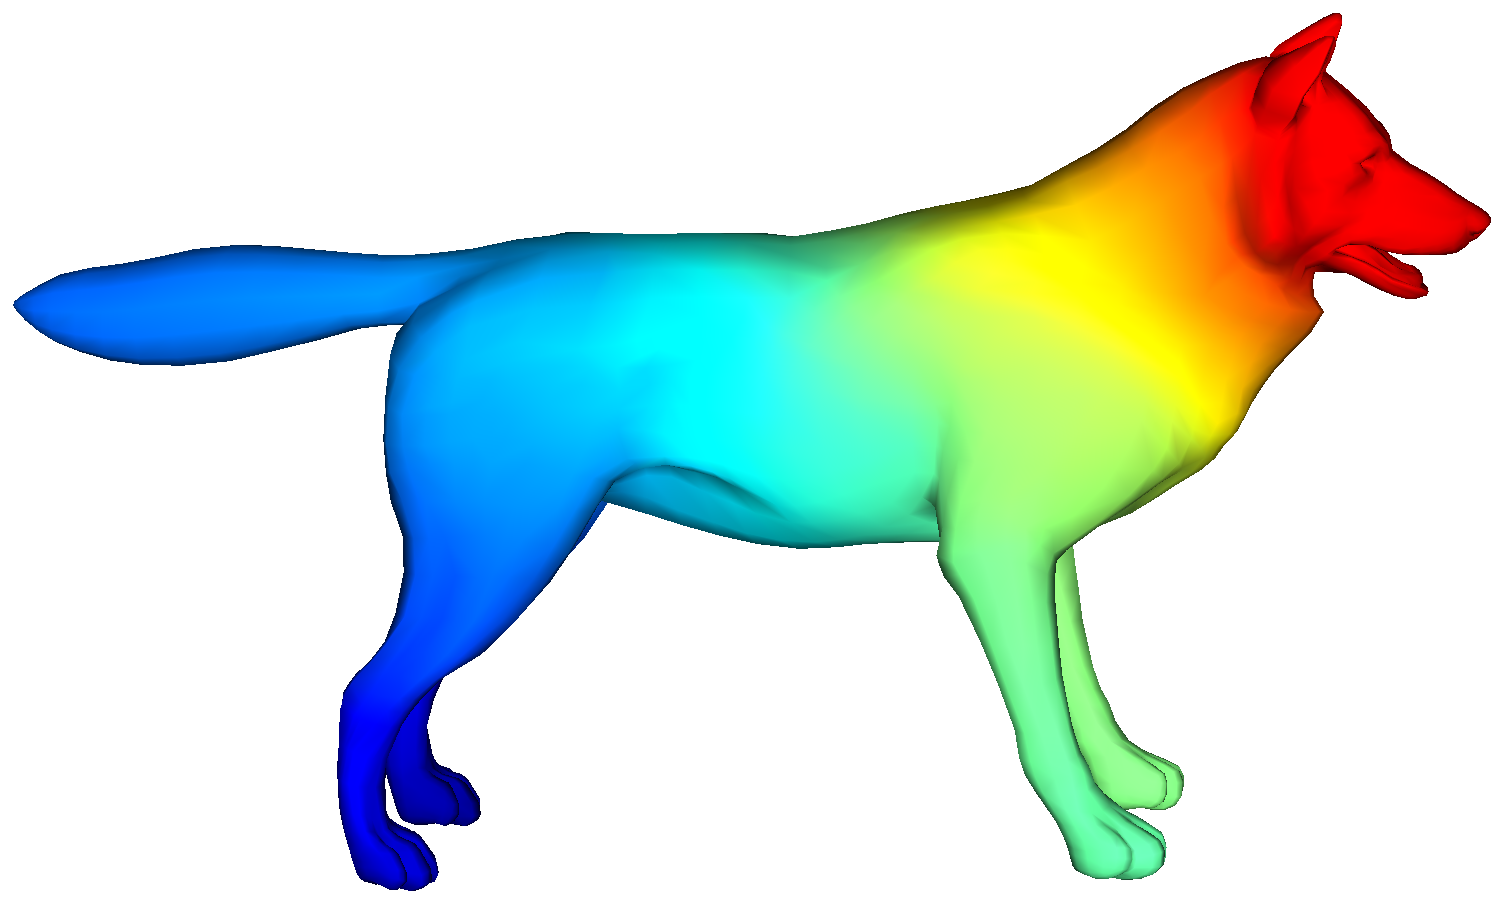
\includegraphics[width=\linewidth]{1}
                \caption{$\chi_1$}
                \label{fig:wolf_mhb_1}
        \end{subfigure}%
        ~
        \begin{subfigure}[b]{0.3\linewidth}
                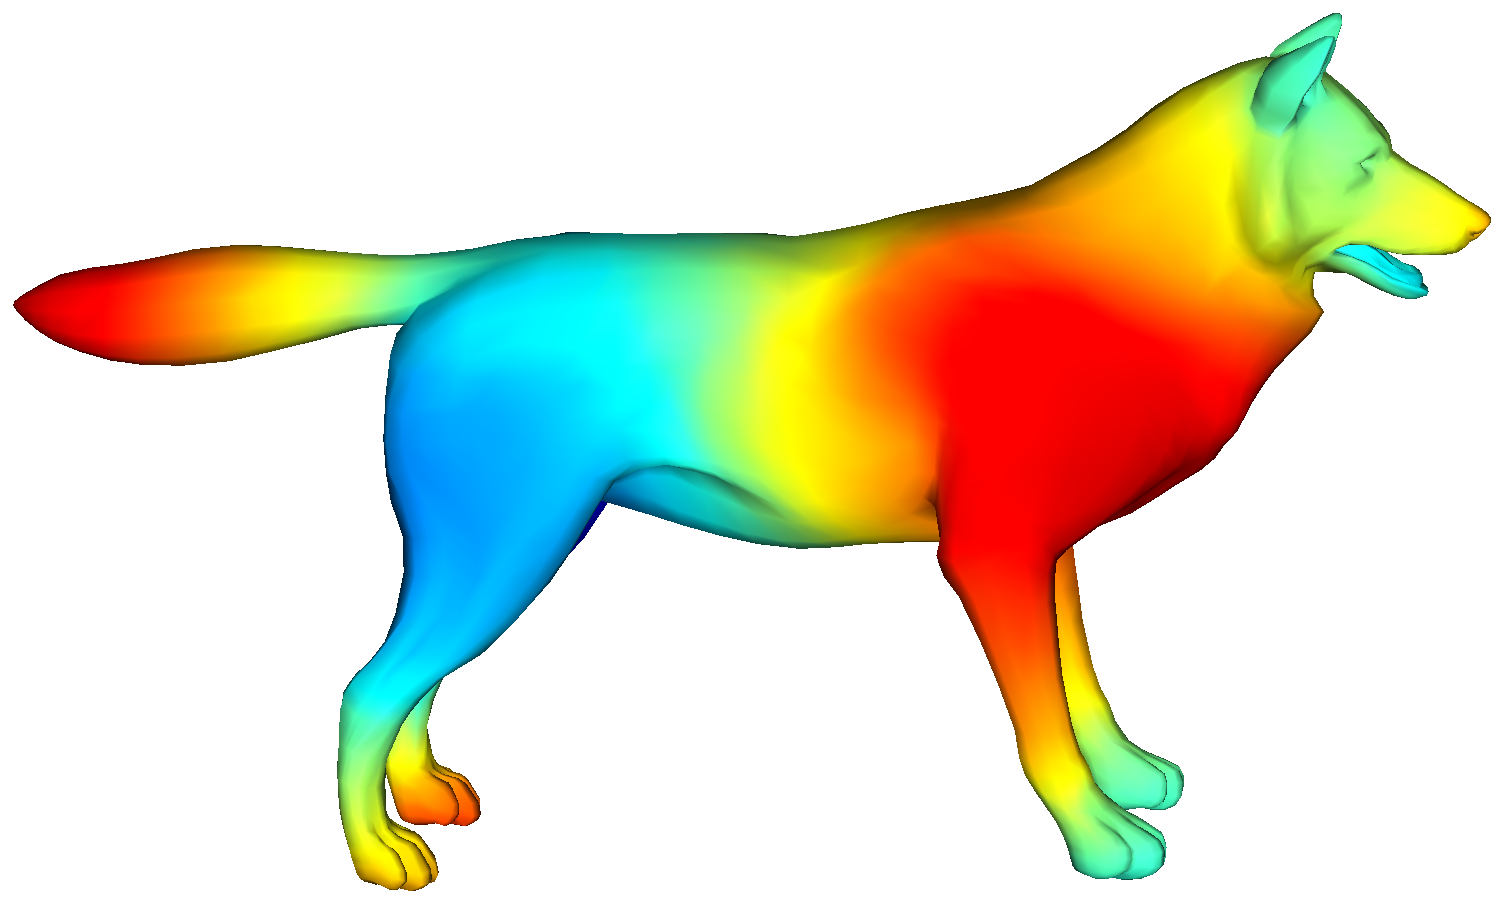
\includegraphics[width=\linewidth]{2}
                \caption{$\chi_{10}$}
                \label{fig:wolf_mhb_10}
        \end{subfigure}
        ~
        \begin{subfigure}[b]{0.3\linewidth}
                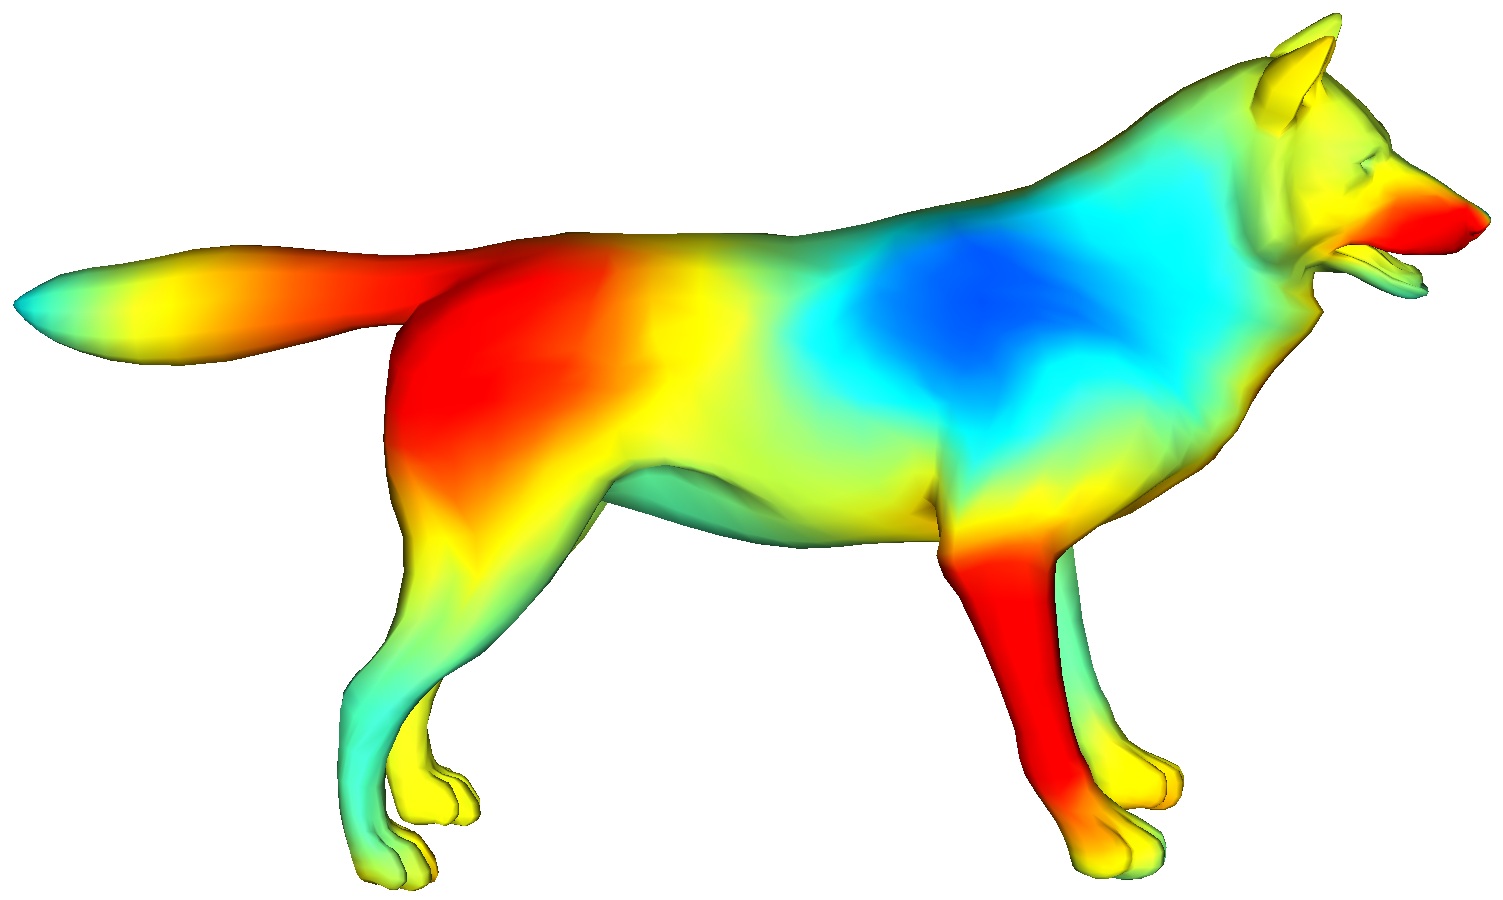
\includegraphics[width=\linewidth]{3}
                \caption{$\chi_{20}$}
                \label{fig:wolf_mhb_20}
        \end{subfigure}
        \caption[Visualization of MHBs.]
        {Visualization of the Laplacian eigenfunctions (MHB).
         From left to right, the first, tenth, and twentieth
         eigenfunctions are highlighted.}
        \label{fig:mhb}
\end{figure}

\subsection{Spectral Mesh Approximation via MHB}
\label{sec:mhbapprox}

The MHB can be employed to define the graph Fourier transform, also
known as the \emph{manifold harmonic transform} (MHT), which converts
a function between spatial domain and frequency domain. Any $f\in
L^2(M)$ can be expanded by MHB as
\begin{equation}
\label{eq:mht}
f = \sum_{k=0}^{n-1}\widehat{f}_k\phi_k = \sum_{k=0}^{n-1}\langle f,\phi_k\rangle\phi_k,
\end{equation}
in which $\widehat{f}_k$ is the $k$-th MHT coefficient of $f$.

The MHT is the theoretical foundation of the spectral mesh compression
proposed by Karni and Gotsman~\cite{Karni2000}. Viewing the
Euclidean mesh coordinates $\mathbf{x}$, $\mathbf{y}$ and $\mathbf{z}$
as functions defined on vertices, the basic idea of spectral
compression is to compute the MHT of the coordinate function and then
truncate out certain number of high-frequency coefficients. Take the
x-coordinate function $\mathbf{x}$ as an example. The original
coordinates can be perfectly recovered as in Eq.~(\ref{eq:mht}) if all
$n$ MHT coefficients $\{\widehat{x}_0,\ldots,\widehat{x}_{n-1}\}$ are
used. If we only retain the first $n'<n$ coefficients, the
reconstructed x-coordinate function $\mathbf{x'}=\sum_{k=0}^{n'-1}
\widehat{x}_k\phi_k$ is a low-pass-filtered version of $\mathbf{x}$
and can be regarded as an acceptable approximation. The reconstructed
mesh is smooth and the overall appearance tends to be very similar to
the original mesh, since low-frequency components, which correspond to
large-scale shape information, are prioritized to be preserved, and
our visual observations tend to be more forgiving to the loss of
high-frequency information.

Fig.~\ref{fig:fourier_approx} shows an example result of
spectral approximation using different number of MHB.
\begin{figure}
 \centering
 \begin{subfigure}[b]{0.23\linewidth}
  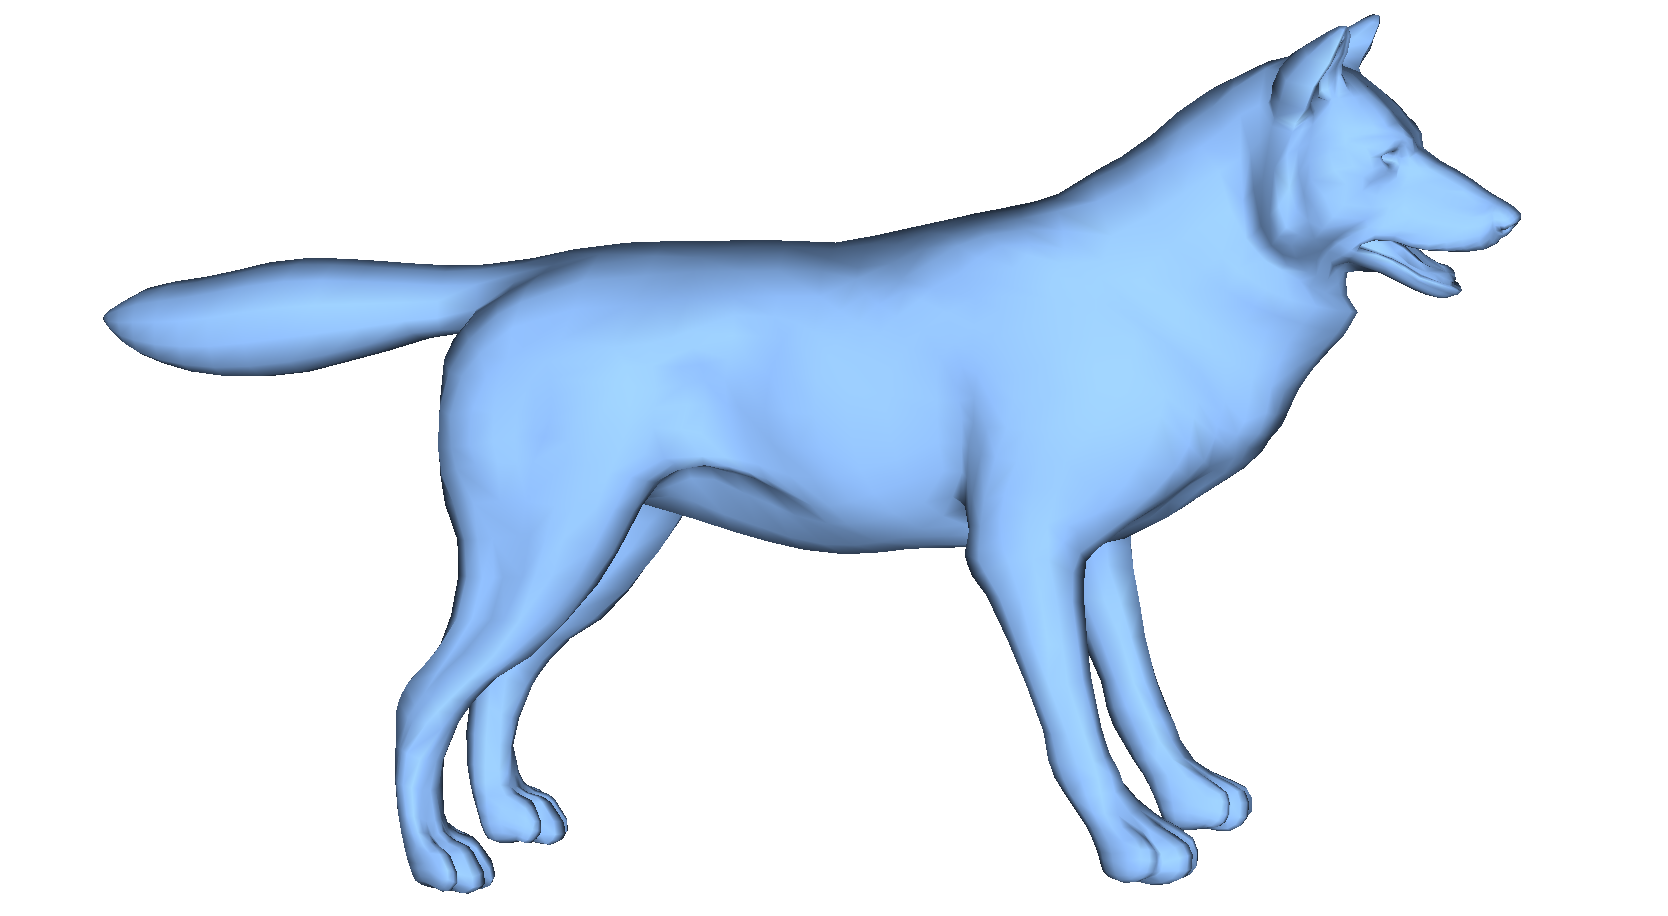
\includegraphics[width=\linewidth]{4}
  \caption{}
  \label{fig:fourier1}
 \end{subfigure}
 ~
 \begin{subfigure}[b]{0.23\linewidth}
  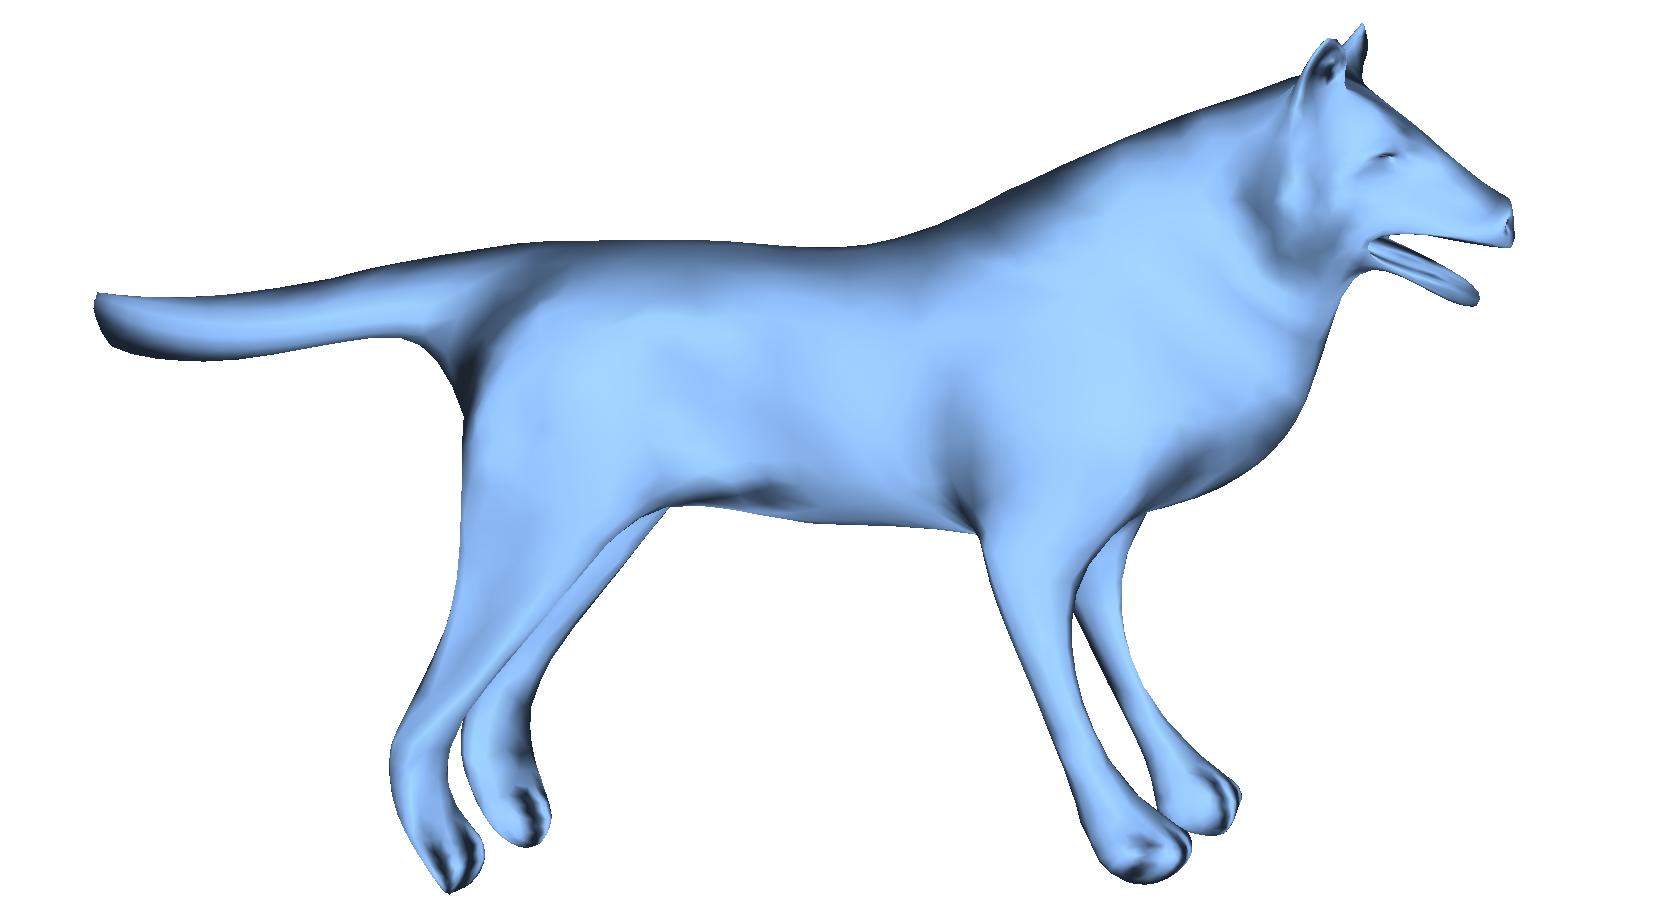
\includegraphics[width=\linewidth]{5}
  \caption{}
  \label{fig:fourier2}
 \end{subfigure}
 ~
 \begin{subfigure}[b]{0.23\linewidth}
  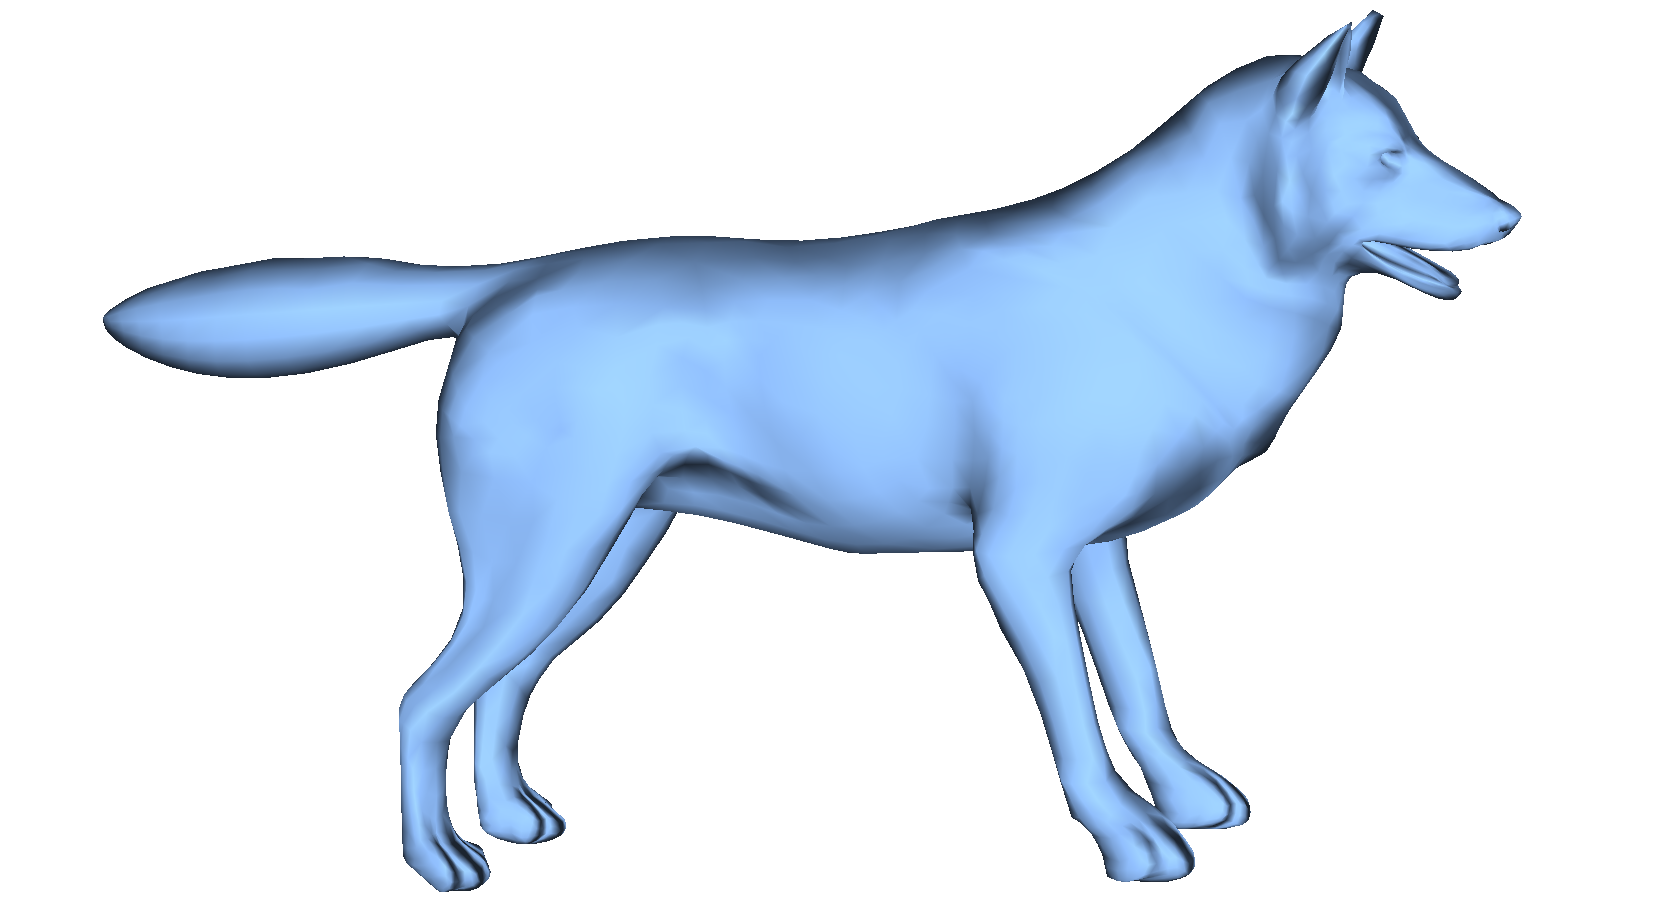
\includegraphics[width=\linewidth]{6}
  \caption{}
  \label{fig:fourier3}
 \end{subfigure}
 ~
 \begin{subfigure}[b]{0.23\linewidth}
  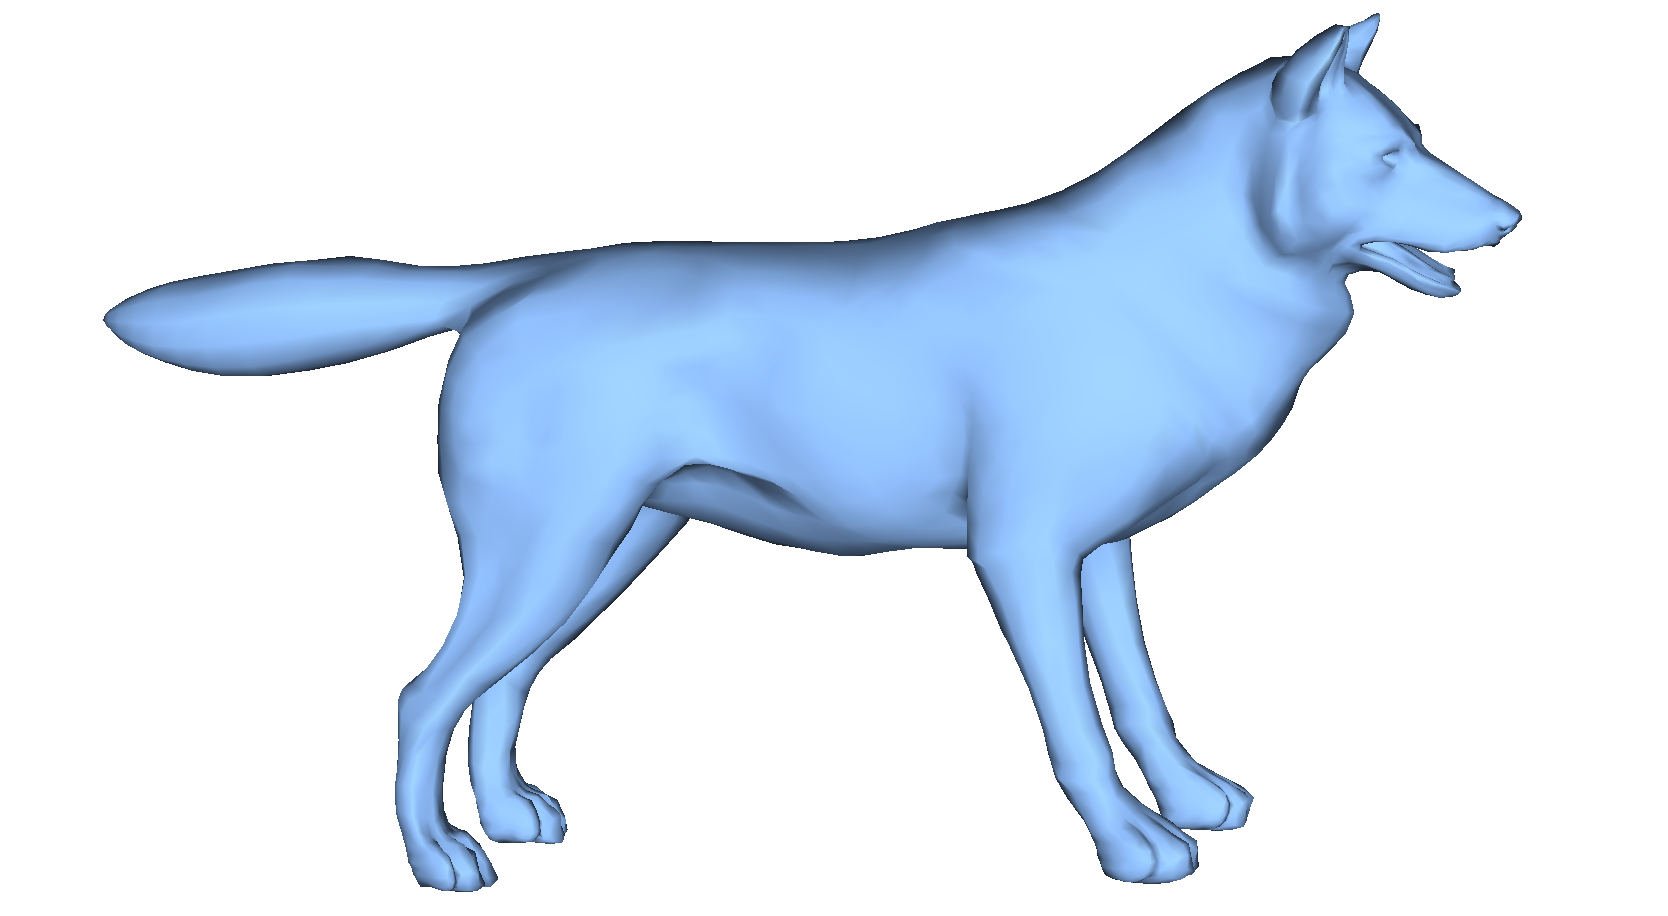
\includegraphics[width=\linewidth]{7}
  \caption{}
  \label{fig:fourier4}
 \end{subfigure}
 \caption[Spectral approximation of wolf model.]
 {Spectral approximation~\cite{Karni2000} of a 3D
  wolf model containing 4,344 vertices. (a) The original mesh. (b)
  Reconstruction using 100 eigenbases. (c) Reconstruction using 300
  eigenbases. (d) Reconstruction using 1000 eigenbases.}
 \label{fig:fourier_approx}
\end{figure}

\subsection{Spectral Graph Wavelets}
\label{sec:sgw}

The spectral graph wavelets (SGW), as described
in~\cite{Hammond2011}, are expressed as bivariate kernel
functions expanded on the MHB
\begin{equation}
\mathbf{\Psi_t}(i,j)=\sum_{k=0}^{n-1}g(t\lambda_k)\chi_k(i)\chi_k(j),
\end{equation}
where $g$ is the real-valued wavelet generator function and $t$ is the
scale parameter. The generator function $g$ modulates the spectral
wavelets in the frequency domain, and should satisfy the admissibility
condition
\begin{equation}
C_g=\int_0^{\infty}\frac{g^2(x)}{x}dx < \infty
\end{equation}
and $g(0)=0$. The $i$th row of $\Psi_t$
\begin{equation}
\psi_{t,i}(\cdot)=\sum_{k=0}^{n-1} g(t\lambda_k)\chi_k(i)\chi_k(\cdot)
\end{equation}
is the spectral wavelet spatially-localized at $v_i$, and in the
frequency domain, localized at scale $t$.

In practice, the scale parameter $t$ is discretized. The
spectral graph wavelets $\psi_{t,i}$ are near orthogonal to
$\chi_k$ for $\lambda_k$ near 0, i.e., low-frequency eigenbasis,
for any discrete scale $t$. Hence, to better capture low-frequency signal
information, \cite{Hammond2011} also introduced the \emph{spectral
scaling functions} which have similar constructions with SGW but act like low-pass filters
\begin{equation}
  \mathbf{\Phi}_t(i,j)=\sum_{k=0}^{n-1} h(t\lambda_k)\chi_k(i)\chi_k(j),
\end{equation}
in which the scaling generator function $h$ should satisfy $h(0)>0$
and $h(x)\rightarrow 0|_{x\rightarrow\infty}$.

Suppose we compute the spectral wavelets at $J$ different scales
$\{t_1,t_2,\ldots,t_J\}$, the constructed SGW then comprises
$(J+1)\times n$ functions in $\mathbb{R}^n$. In this chapter, we adopt
the same formulation of wavelet and scaling functions used
in~\cite{Hammond2011} with the generator function
\begin{equation}
g(x)=
\begin{cases}
        x^2 & \text{if } x<1\\
        -5+11x-6x^2+x^3 & \text{if } 1\leq x \leq 2\\
        4x^{-2} & \text{if } x>2.
    \end{cases}
\end{equation}
The $J$ scales are selected to be logarithmically equally spaced
between the minimum scale $t_J=2/\lambda_{max}$ and the maximum scale
$t_1=40/\lambda_{max}$, where $\lambda_{max}$ is the upper bound of
the Laplacian eigenvalues. For the scaling function, the generator is
$h(x)=\gamma\exp(-(\frac{20x}{0.6\lambda_{max}})^4)$, in which
$\gamma=h(0)$ equals the maximum value of $g$.

Fig.~\ref{fig:sgw} visualizes multiscale spectral graph wavelets on a
3D mesh. It may be noted that, the values of wavelets are attenuated
and oscillating on the mesh, and wavelets with a larger scale have a
wider oscillating window.
\begin{figure}
\centering
\begin{subfigure}[b]{0.3\linewidth}
    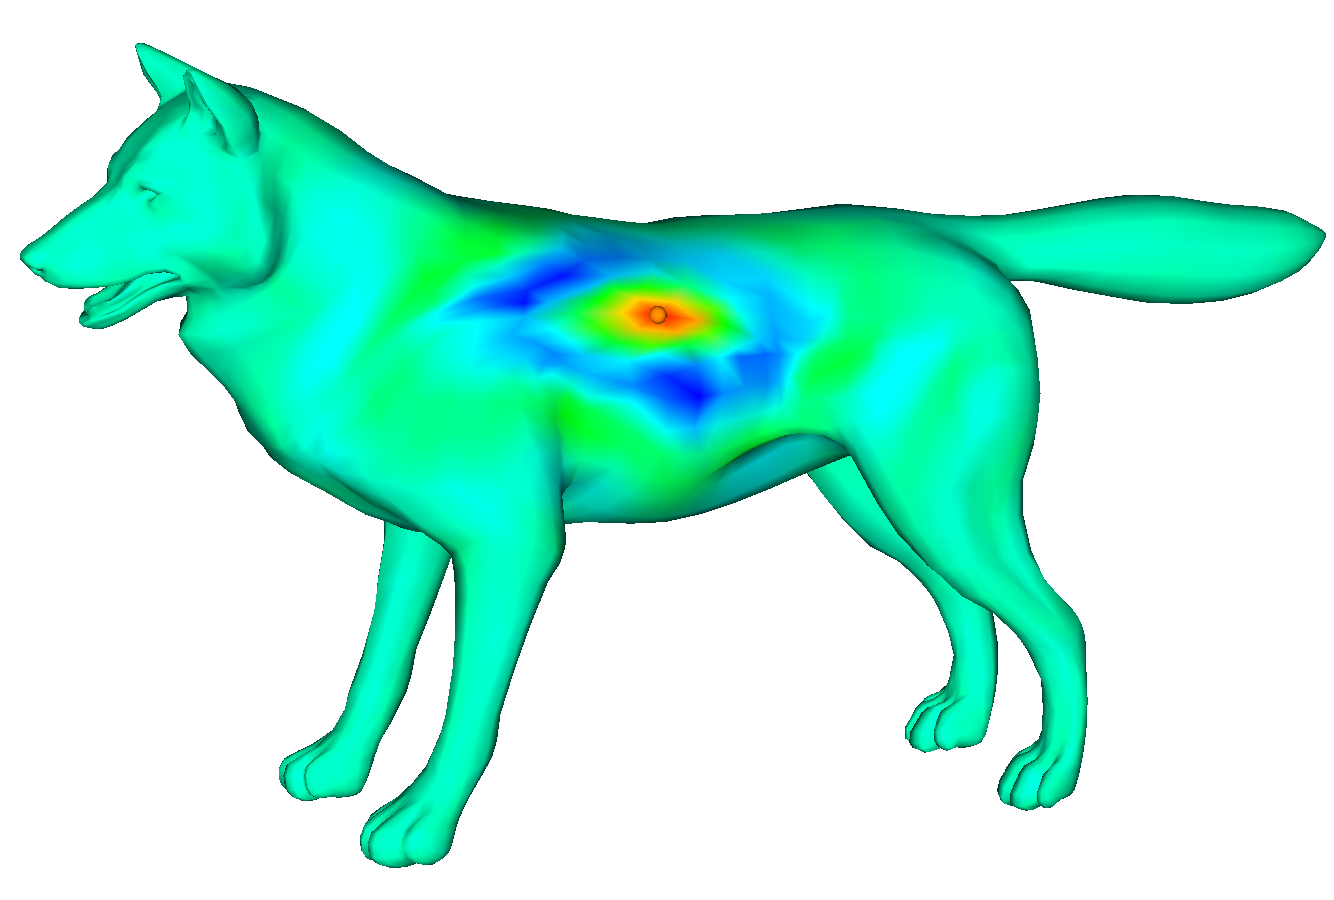
\includegraphics[width=\linewidth]{8}
    \label{fig:sgw1}
\end{subfigure}%
~
\begin{subfigure}[b]{0.3\linewidth}
    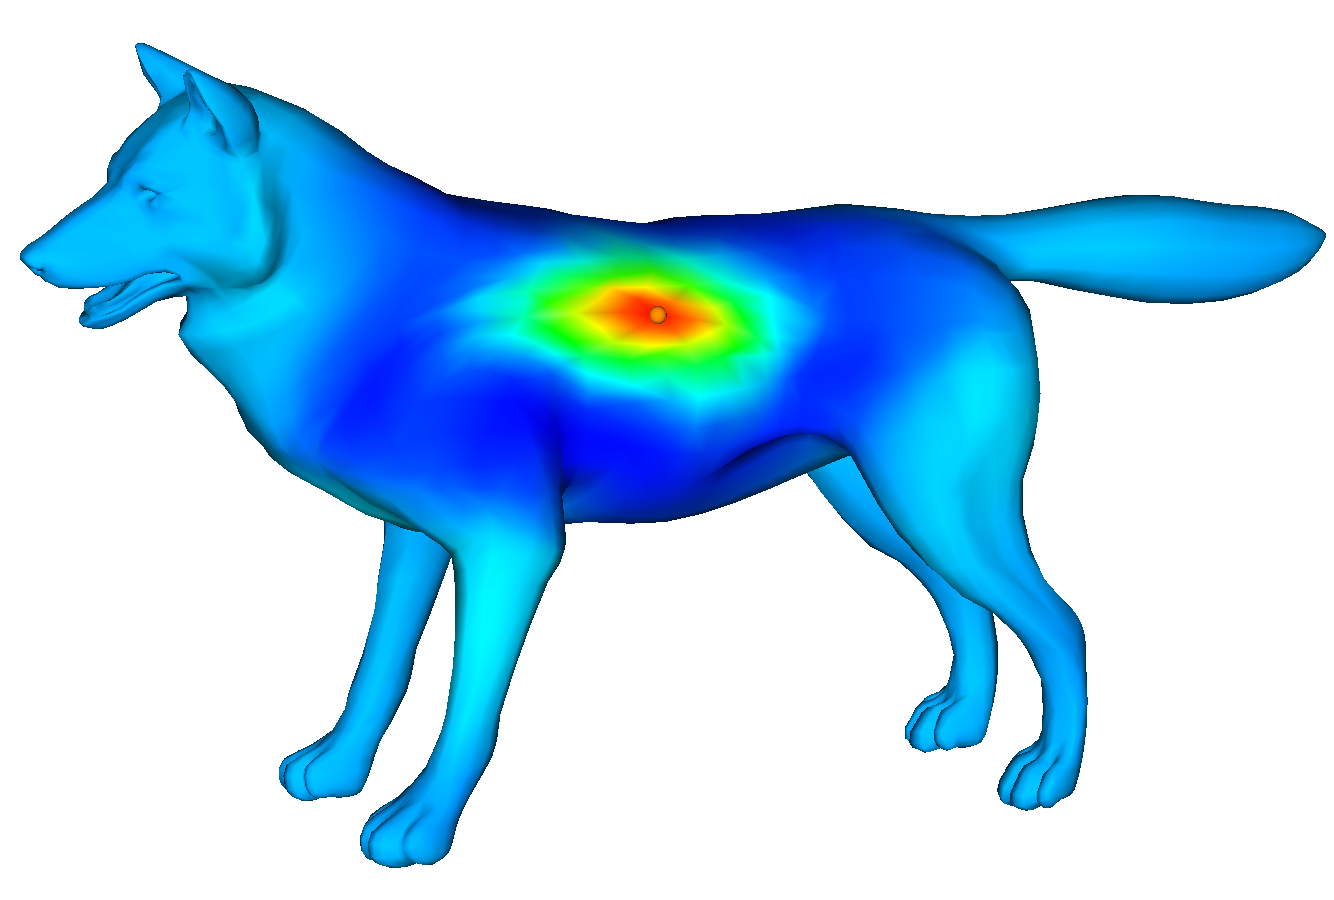
\includegraphics[width=\linewidth]{9}
    \label{fig:sgw2}
\end{subfigure}
~
\begin{subfigure}[b]{0.3\linewidth}
    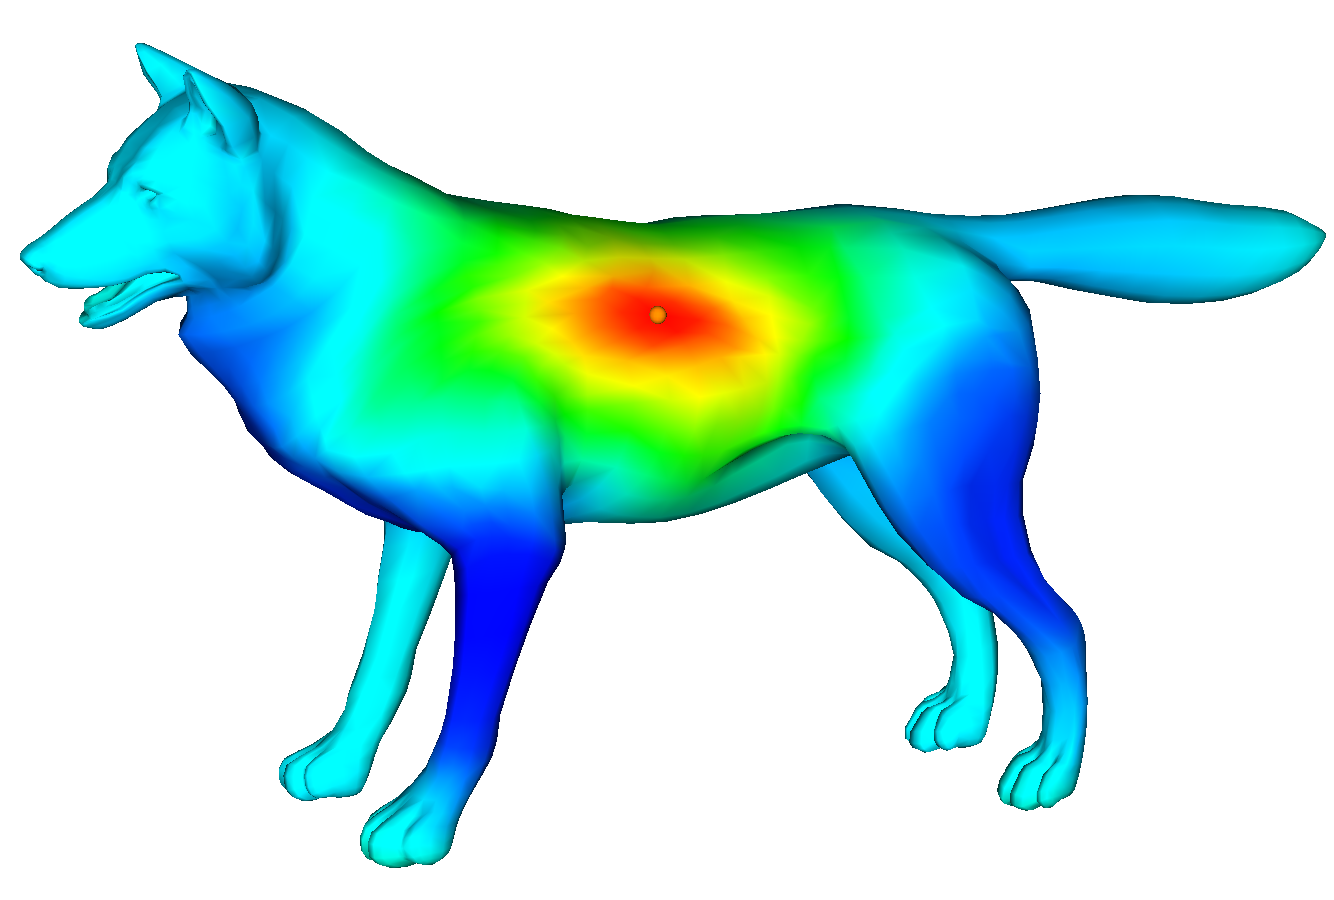
\includegraphics[width=\linewidth]{10}
    \label{fig:sgw3}
\end{subfigure}%
\caption[Visualization of spectral graph wavelets with different scales.]
{Visualization of spectral graph wavelets localized at the
 same point but with different scales. From left to right, the
 spectral wavelets at scale 1, 3, and 5 are highlighted.}
\label{fig:sgw}
\end{figure}

In Sec.~\ref{sec:mhbapprox} we have shown that the mesh coordinates
can be transformed into the frequency domain via MHT using the
Laplacian eigenbasis, and compression can be achieved by trimming out
a user-specified number of high-frequency coefficients. The main
drawbacks of this naive and simple low-pass spectral compression
method are: (1) It innately favors low-frequency information while
most high-frequency geometric details are compromised; (2) The
Laplacian eigenbasis, which serve as the compression dictionary, all
have global support and therefore are not efficient in encoding local
geometry.

In this chapter, we propose to use SGW to construct a redundant
dictionary. Because of its powerful property of spatial localization,
the multiscale SGW functions are much more efficient in representing
local mesh geometry around individual vertices than the Laplacian
eigenbasis. Since the size of SGW dictionary is much larger than the
number of mesh vertices, we employ powerful sparse approximation
algorithms to find a compact representation which selects the most
appropriate basis in the procedure.

\subsection{Sparse Approximation of Mesh Coordinates}

For mesh $M$, let $\mathbf{D}$ be a dictionary of $L^2(M)$ containing
$m$ normalized basis vectors. The dictionary can be written as a
$n\times m$ matrix $\mathbf{D} = \begin{pmatrix} \mathbf{a_1} &
  \mathbf{a_2} & \ldots & \mathbf{a_m} \end{pmatrix}$, where
$\mathbf{a_i} \in \mathbb{R}^{n\times 1}$. Our aim is to approximate
function $\mathbf{y}\in L_2(M)$ with a linear combination of the atoms
in $\mathbf{D}$, expressed in the matrix form as
$\widehat{\mathbf{y}}=\mathbf{D}\mathbf{x}=\sum_{i=1}^m
x_i\mathbf{a_i}$. Here the vector $\mathbf{x}\in\mathbb{R}^m$ is the
coefficient representation of the input signal $\mathbf{y}$ w.r.t. the
dictionary $\mathbf{D}$.

An effective compression of the original signal $\mathbf{y}$ requires
the number of elementary signals that participate in the linear
combination to be small and the reconstructed result
$\widehat{\mathbf{y}}$ to be as close to $\mathbf{y}$ as possible. In
principle, the number of non-zero elements of the coefficient vector
$\mathbf{x}$, denoted by the pseudo-norm $\|\mathbf{x}\|_0$, should
satisfy $\|\mathbf{x}\|_0 \ll n$ in order to achieve significant
reduction in storage. Fixing the number of participating atoms in the
sparse approximation to be $n'$, the problem to produce the optimal
sparse representation $\mathbf{x}$ can be formulated as:
\begin{equation}
  \min_{\mathbf{x}} \|\mathbf{y}-D\mathbf{x}\|_2^2\ \textrm{subject\ to}\ \|\mathbf{x}\|_0 = n'.
\label{eq:sa}
\end{equation}

If the input signal has $c$ channels, denoted as a $n\times c$ matrix
$\mathbf{Y}=(\mathbf{y_1},\mathbf{y_2},\ldots,\mathbf{y_c})$, the
coefficient representation should be a $m\times c$ matrix
$\mathbf{X}=(\mathbf{x_1},\ldots,\mathbf{x_c})$ satisfying $\mathbf{Y}
\approx \mathbf{D}\mathbf{X}$. We may either treat each channel
(column) of $\mathbf{Y}$ independently and select different subsets of
participating atoms for each channel, or use the same subset for all
the channels and minimize the combined approximation errors. The
latter one is called the \emph{simultaneous sparse approximation} problem
\begin{equation*}
  \min_{\mathbf{X}} \|\mathbf{Y}-\mathbf{D}\mathbf{X}\|_F^2
\end{equation*}
subject to
\begin{equation}
\begin{cases}
    support(\mathbf{x_1})=\cdots=support(\mathbf{x_c})\\
    \|\mathbf{x_1}\|_0=\cdots=\|\mathbf{x_c}\|_0=n',
\end{cases}
\label{eq:simulsa}
\end{equation}
where $\|\cdot\|_F$ is the Frobenius norm, and $support(\mathbf{x_i})$
denotes the index set of non-zero elements in $\mathbf{x_i}$.

The vertex coordinates of a mesh can be treated as a 3-channel signal
$p(\mathbf{v})=(\mathbf{v_x}, \mathbf{v_y}, \mathbf{v_z})$. Since the
three coordinate functions are correlated, it is preferable to
formulate the mesh compression as the simultaneous sparse
approximation problem. Determining the optimal solution to
Eq.~(\ref{eq:simulsa}) is NP-hard, but we can find approximate
solutions using greedy pursuit algorithms such as the
\emph{simultaneous orthogonal matching pursuit} (S-OMP)
\cite{Tropp2006a}. The key idea is to iteratively select
from the dictionary a new atom that has the best correlation with the
residual shape, and then project the original mesh onto the space
spanned by the selected atoms to obtain a new approximate shape.
Please refer to Algorithm~\ref{alg:somp} for details.
\begin{algorithm}
\caption{S-OMP on 3D mesh coordinates.}
\label{alg:somp}
\begin{algorithmic}
\STATE \textbf{Input:}
\STATE \begin{itemize}
         \item 3D mesh coordinates $\mathbf{S}\in\mathbb{R}^{n\times 3}$.
         \item Dictionary $\mathbf{D}=\{\mathbf{a_1},\mathbf{a_2},\ldots,\mathbf{a_m}\}, \mathbf{a_i}\in\mathbb{R}^3$.
         \item The number of atoms to be selected $n'$.
       \end{itemize}
\STATE \textbf{Initialization:}
\STATE \begin{itemize}
         %\item The index set of all atoms $\Omega=\{1,2,\ldots,m\}$.
         \item The initial index set of selected atoms $\Lambda_0=\emptyset$.
         \item The initial residual $\mathbf{R_0}=\mathbf{S}$;
         \item The iteration counter $t=1$.
       \end{itemize}
\STATE \textbf{Procedure:}
\STATE (1) Find an index $i_t$ of $\mathbf{D}$ that satisfies
    $$ i_t = \argmax_{j\not\in\Lambda_{t-1}} \sum_{k=1}^3 |\langle \mathbf{R_{t-1}}\mathbf{e_k}, \mathbf{a_j} \rangle|, $$
    where $e_k$ denotes the $k$th canonical basis vector in $\mathbb{R}^3$.
\STATE (2) Set $\Lambda_t=\Lambda_{t-1}\bigcup\{i_t\}$.
\STATE (3) Compute the coefficient matrix $\mathbf{C_t}$ by solving the least-square problem
    $$ \mathbf{C_t}=\argmin_{\mathbf{X}}=\|\mathbf{S}-\mathbf{D}\mathbf{\mathbf{X}}\|_2^2$$
    subject to $support(X)=\Lambda_t.$
\STATE (4) Calculate the new approximation and residual:
    $$ \mathbf{\widehat{S}_t} = \mathbf{D}\mathbf{C_t}, $$
    $$ \mathbf{R_t} = \mathbf{S} - \mathbf{\widehat{S}_t}. $$
\STATE (5) Stop if $t=n'$. Otherwise, increment $t$ and go to (1).
\STATE \textbf{Output:}
\STATE \begin{itemize}
         \item The index set of selected atoms $\Lambda_{n'}$.
         \item Final coefficient matrix $\mathbf{C_{n'}}$.
        \end{itemize}
\end{algorithmic}
\end{algorithm}

We may also adopt the \emph{simultaneous matching pursuit} (S-MP) algorithm
which can be viewed as a simplification of S-OMP. The main difference from S-OMP is
the omission of the step to update all existing coefficients by orthogonal projection.
If all atoms in $\mathbf{D}$ are mutually orthogonal (e.g., Fourier dictionary), S-MP and S-OMP
will produce exactly the same result.

\subsection{Dictionary Design Strategies}
\label{sec:dictionary}

The key to effective sparse approximation is the selection of
elementary functions that form the dictionary. A natural choice is the
MHB dictionary composed entirely of Laplacian eigenbasis
$\{\chi_0,\chi_2,\ldots,\chi_{n-1}\}$. The MHB functions have global
support and multiple frequencies, making the MHB dictionary a good
choice for encoding a shape when global, periodical, and symmetric
information is prioritized to be preserved. In addition, since MHB are
orthogonal basis, we can replace orthogonal matching pursuit (OMP)
with the much faster matching pursuit (MP) and the approximation
results will be the same.

However, MHB dictionary is very inefficient in capturing
non-periodical, local details due to the global support. It is
desirable to have a dictionary with a class of functions that have
local support but are still smooth and multiscale. In this work, we
propose to use normalized multiscale SGW, as described in
Sec.~\ref{sec:sgw}, as atoms to construct the dictionary for sparse
approximation. The SGW dictionary has several advantages:
\begin{itemize}
\item The SGW atoms are compact and localized at vertices, suitable
  for encoding local geometric features.
\item The SGW atoms can cover multiple scales, enabling the efficient
  representation of both small-scale and large-scale shape information
  in the vincinity of each vertex.
\item The computation of SGW from MHB is straightforward, and can be
  done on the decoder side provided the mesh connectivity is known.
\end{itemize}

On the flip side, the SGW are less efficient than MHB for encoding
global shape structures. Moreover, since SGW functions always have
extreme values at their origin vertices, a mesh reconstructed from SGW
atoms may exhibit unpleasant protrudes at vertices where selected SGW
are centered, which can be further ameliorated by constructing a
dictionary that contains both MHB and SGW. The mixed dictionary
potentially inherits the advantages of both waveforms, at the cost of
increased dictionary size.

The SGW or SGW+MHB dictionary are non-orthogonal and redundant,
forcing us to use costly sparse approximation methods such as S-OMP.
The enlarged dictionary also increase the storage requirements for the
dictionary themselves and for the sparse coefficient representation
(see Sec.~\ref{sec:compratio}).

Fig.~\ref{fig:wolf} shows an example of sparse approximation results
using three methods: (1) Spectral mesh compression via MHB, as
described in Sec.~\ref{sec:mhbapprox}; (2) S-MP with the MHB
dictionary; (3) S-OMP with the SGW dictionary. In this example, the
S-MP method produces higher-quality shape approximation than the naive
low-pass spectral approximation using the same MHB dictionary.
Adopting the multiscale SGW dictionary in place of MHB further
improves the approximation results. In particular, the SGW dictionary
are more effective in preserving local geometric features, while
MHB-based approximations have the tendency to smooth out some body
parts such as the wolf's legs when the number of participating bases
is small.

\begin{figure}
    \centering
    \includegraphics[width=\linewidth]{11}
    \caption[Comparison of three approximation methods.]
    {Comparison of the approximation results of three
      different approximation methods. \emph{Top row}: Spectral
      compression by truncating MHB coefficients. \emph{Second row}:
      S-MP approximation with MHB bases. \emph{Bottom row}: S-OMP
      approximation with SGW bases. For each method, from left to
      right, the number of participating bases are 20, 50, and 100,
      respectively.}
    \label{fig:wolf}
\end{figure}

\subsection{Compression Ratio and Analysis}
\label{sec:compratio}

Now we analyze the compression ratio of the simultaneous sparse
representation using a simple coding scheme. Assume the dictionary $D$
are known in advance on both the encoder and decoder sides. The sparse
$m\times 3$ coefficient matrix $\mathbf{X}$ contains $n'$ non-zero
rows, and can be conveniently expressed by $3n'$ non-zero values and a
vector of size $n'$ specifying the indices of corresponding atoms. For
a dictionary containing $m$ atoms, each index occupies $\lceil\log_2
m\rceil$ bits, and the total cost to store the index vector is
$n'\lceil\log_2 m\rceil$. If the sparsity of $\mathbf{X}$, namely the
ratio of non-zero elements, is greater than $1/\lceil\log_2 m\rceil$,
it would be more efficient to represent the non-zero positions with a
bit-vector of size $m$. Assuming each signal element in $\mathbf{Y}$
takes up $k$ bits, and each coefficient in $\mathbf{X}$ requires $k'$
bits to store, the storage size of the original 3D coordinates is then
$3nk$ bits. The effective compression ratio is
\begin{equation}\label{eq:compress}
\Gamma = \frac{3n'k' + \min (m, n'\lceil\log_2 m\rceil}{3nk}.
\end{equation}

Assume that the dictionary contains $m=\alpha n$ atoms, and both the
coordinates and coefficients are stored in single-precision $k=k'=32$,
the compression ratio is then
\begin{equation}\label{eq:compress2}
  \Gamma = \frac{n'}{n} + \min(\frac{\alpha}{96}, \frac{n'\lceil\log_2\alpha n\rceil}{96n}).
\end{equation}
In comparison, the compression ratio of the coefficient truncation
method introduced in Sec.~\ref{sec:mhbapprox} is simply $n'/n$ with
$n'$ coefficients, since there is no need to store the indices of
non-zeros.

From Eq.~(\ref{eq:compress2}) we can easily see that enlarging the
dictionary (larger $\alpha$) increases the overhead ratio for a given
mesh. In addition, when the coefficient matrix is very sparse, the
overhead ratio becomes smaller for larger meshes, since $log_2\alpha
n$ increases slower than $n$.

\subsection{Mesh Partitioning}

The most time-consuming part of S-OMP is to compute the maximum inner
product between the residual and available atoms, which costs $O(mn)$
in each iteration. In principle, the required number of iterations
$n'$ and the size of dictionary $m$ are linearly proportional to the
mesh size $n$, hence the total time complexity is $O(n^3)$, which is
unacceptable for very large meshes. In addition, all the dictionaries
we use are constructed from the eigenvectors of mesh Laplacian, but
the full Laplacian eigendecomposition of a large mesh is very time
consuming and can be numerically instable. Hence, when the input mesh
is very large, it is necessary to perform graph partitioning and carry
on the compression algorithm on each individual sub-mesh. As suggested
in~\cite{Karni2000}, we use the METIS package~\cite{karypis1998fast}
which implements several fast graph partitioning algorithms.

On the other hand, as mentioned in Sec.~\ref{sec:compratio}, the
overhead for storing the indices of selected atoms is smaller when the
mesh size becomes larger. Moreover, increasing the number of
sub-meshes also increases the occurrences of unpleasant artifacts
along sub-mesh boundaries. Thus, a tradeoff needs to be made between
the compression time and quality. In our implementation, a large mesh
is decomposed into a number of patches containing approximately equal
number of vertices, with the maximum patch size set to be 1,000.


\section{Experimental Results}

\subsection{Evaluation Method}

To evaluate the effectiveness of lossy mesh compression methods, we
adopt the mesh comparison metric proposed
in~\cite{Karni2000} to measure the errors between the
original mesh geometry and approximate ones. Let $M_1$ and $M_2$ be
two meshes to be compared, both containing $n$ vertices, and
$\mathbf{v^1_i}$ and $\mathbf{v^2_i}$ denote the 3D coordinates of the
$i$-th vertex in $M_1$ and $M_2$, respectively. The \emph{geometric
  error} between $M_1$ and $M_2$ is
\begin{equation}
  \|M_1-M_2\|_g = \sum_{i=1}^n \frac{1}{n}\|{\mathbf{v^1_i}-\mathbf{v^2_i}}\|_2.
\end{equation}
To better capture visual closeness such as smoothness,
\cite{Karni2000} introduces another metric which measures
the errors after applying the geometric Laplacian to mesh coordinates,
i.e., transforming the absolute coordinates to differential coordinates
\begin{equation}
  GL(\mathbf{v_i})=\mathbf{v_i}-\frac{\sum_{j\in N(i)}l_{ij}^{-1}\mathbf{v_j}}{\sum_{j\in N(i)}l_{ij}^{-1}},
\end{equation}
where $l_{ij}$ represents the edge length between $v_i$ and $v_j$. The
\emph{differential error} between $M_1$ and $M_2$ is then defined as
\begin{equation}
  \|M_1-M_2\|_d=\sum_{i=1}^n \frac{1}{n}\|GL(\mathbf{v^1_i})-GL(\mathbf{v^2_i})\|_2.
\end{equation}
The final error metric is the average of geometric error and
differential error
\begin{equation}
\|M_1-M_2\|=\frac{1}{2}(\|M_1-M_2\|_g + \|M_1-M_2\|_d).
\label{eq:metric}
\end{equation}

\subsection{Compression Performance}

\begin{figure}
    \centering
    \begin{subfigure}{0.4\linewidth}
        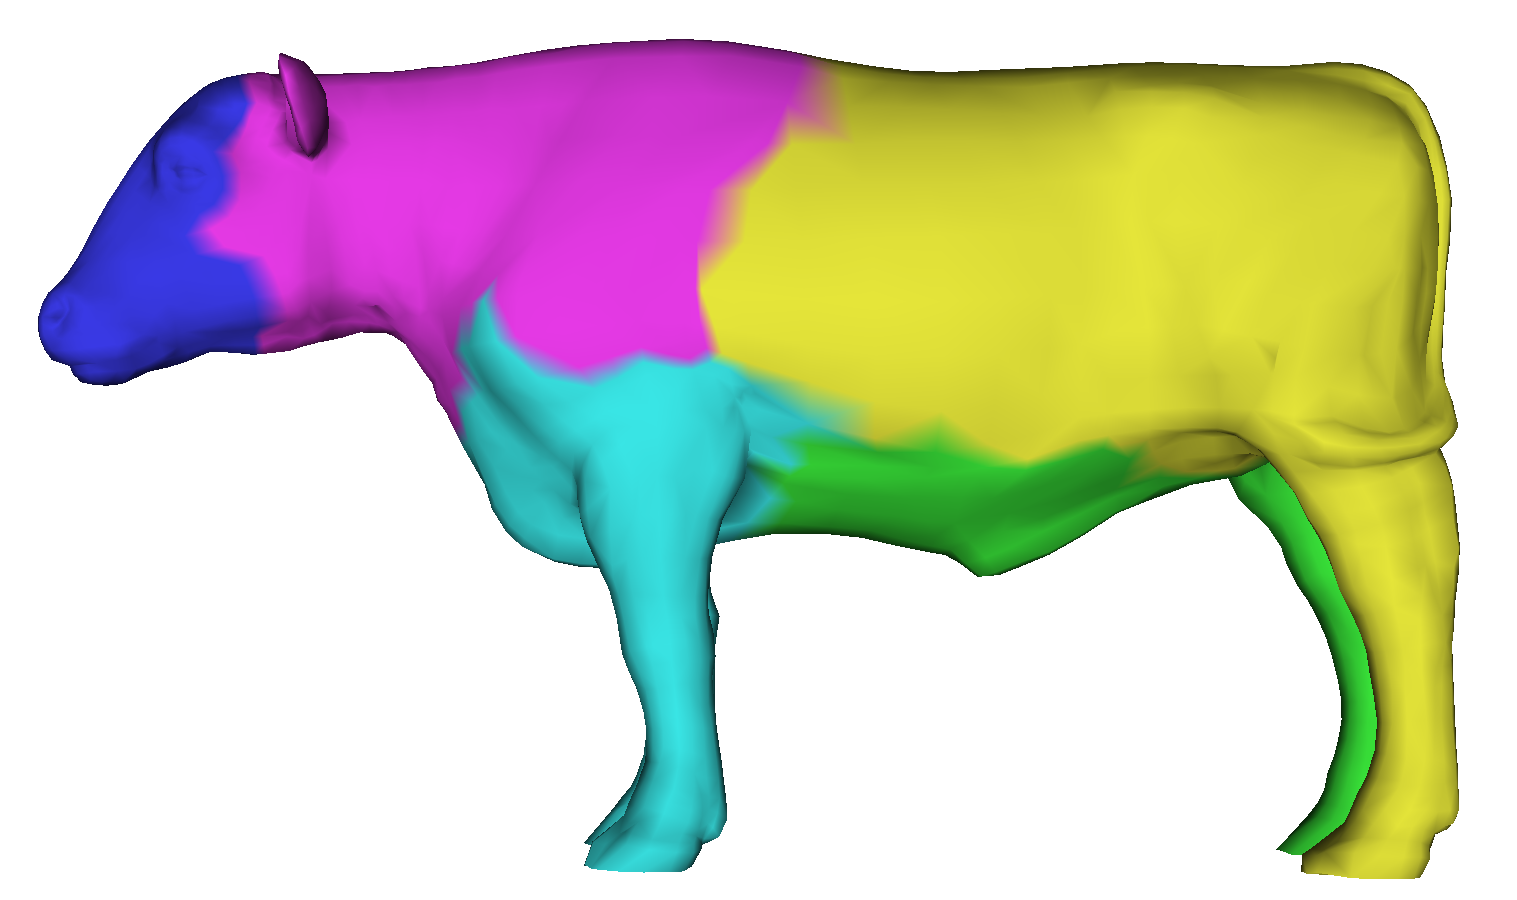
\includegraphics[width=\linewidth]{12}
        \caption{}
    \end{subfigure}
    ~
    \begin{subfigure}{0.4\linewidth}
        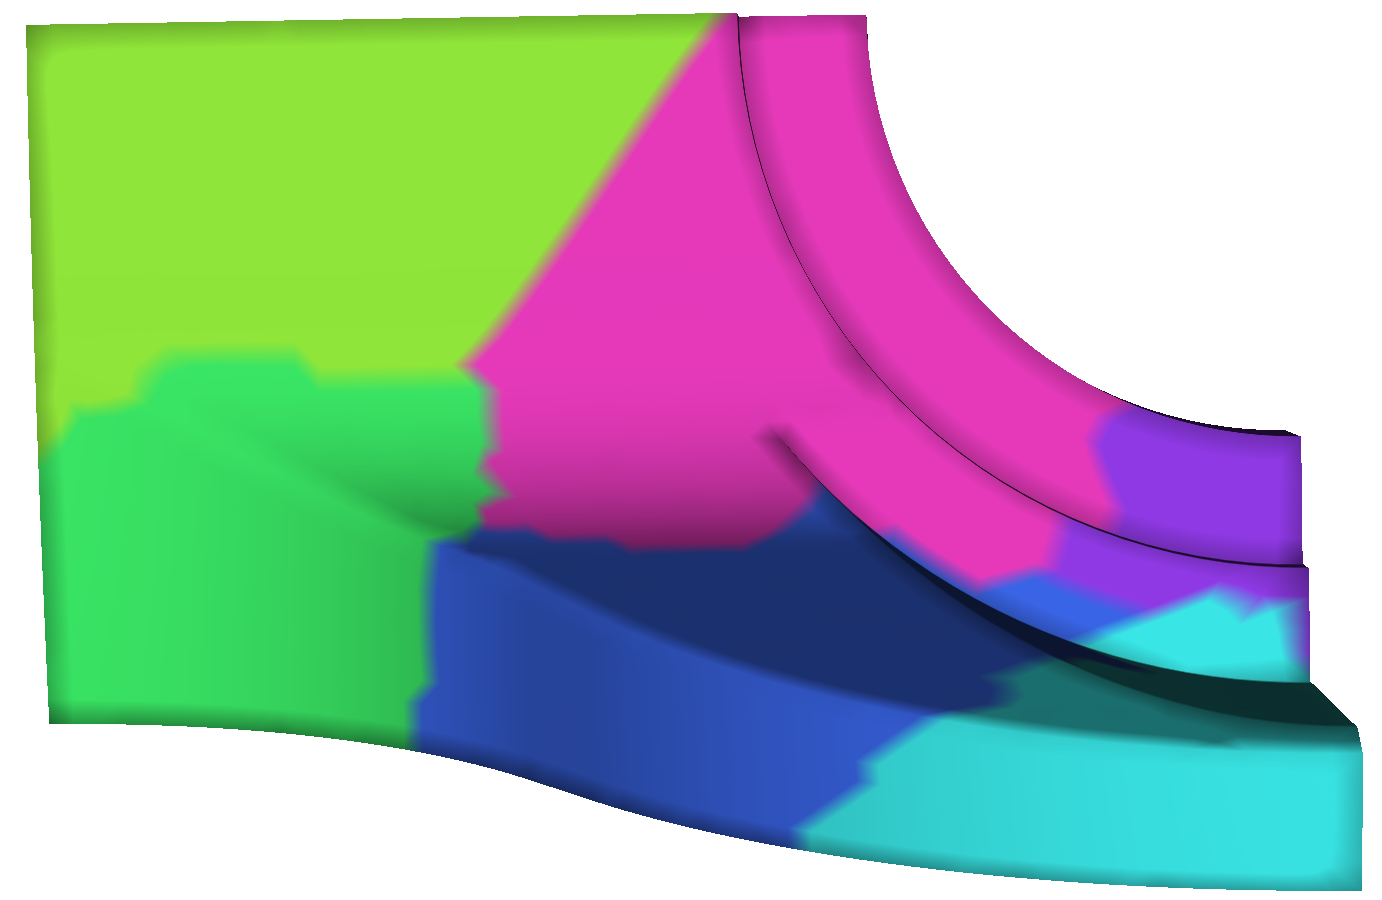
\includegraphics[width=\linewidth]{13}
        \caption{}
    \end{subfigure}
    ~
    \begin{subfigure}{0.4\linewidth}
        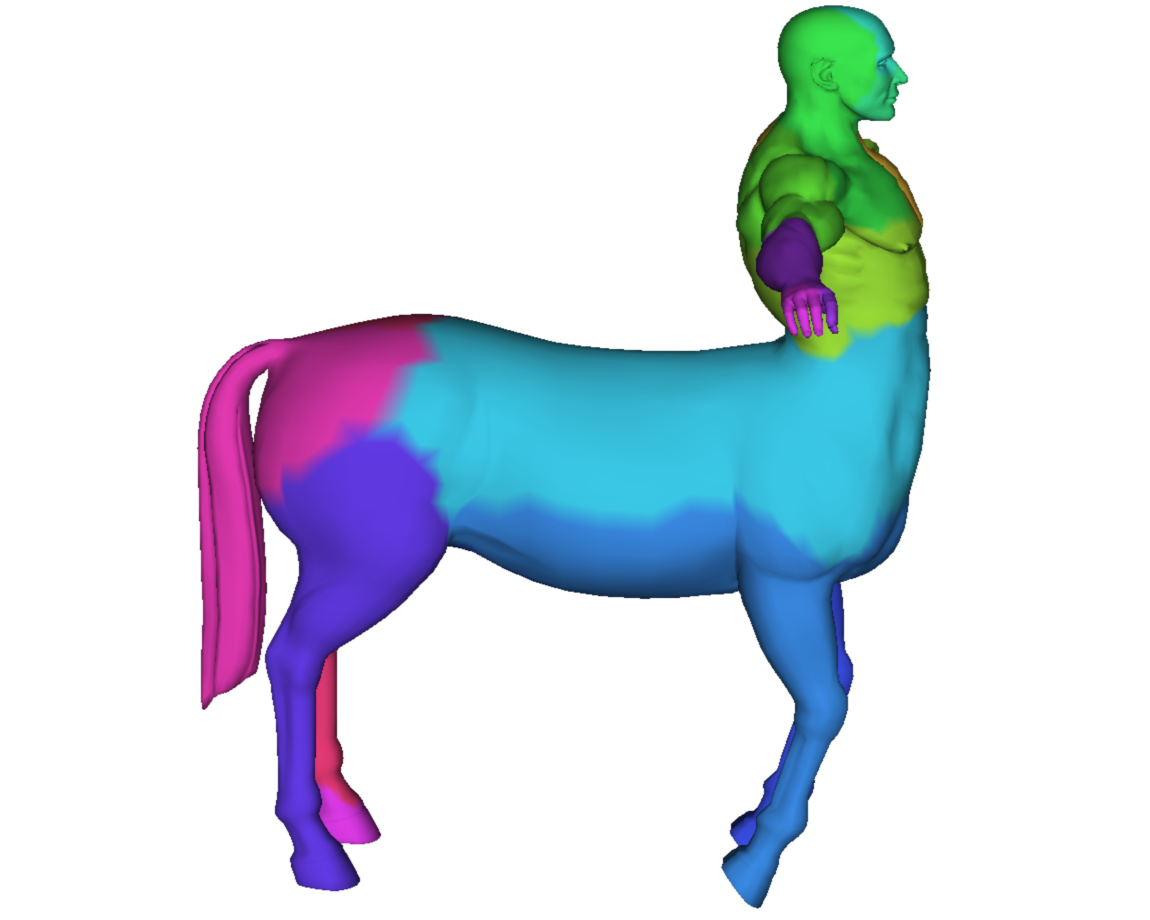
\includegraphics[width=\linewidth]{14}
        \caption{}
    \end{subfigure}
    ~
    \begin{subfigure}{0.4\linewidth}
        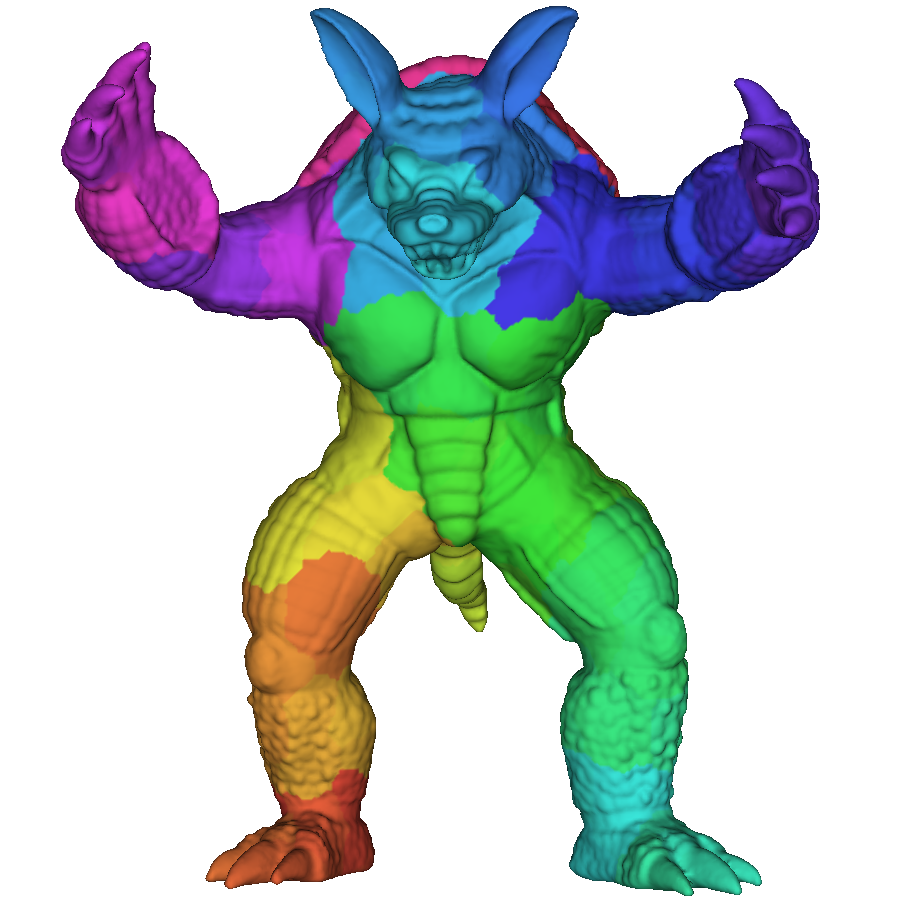
\includegraphics[width=\linewidth]{15}
        \caption{}
    \end{subfigure}
    \caption[Examples of Mesh partitioning.]
    {Models used in our experiments and their
     partitioning. (a) \emph{Cow}: 4,315 vertices. (b)
     \emph{Fandisk}: 6,475 vertices. (c) \emph{Centaur}: 15,768
     vertices. (d) \emph{Armadillo}: 172,974 vertices.}
    \label{fig:partitions}
\end{figure}

\begin{figure}
    \centering
    \begin{subfigure}{0.44\linewidth}
        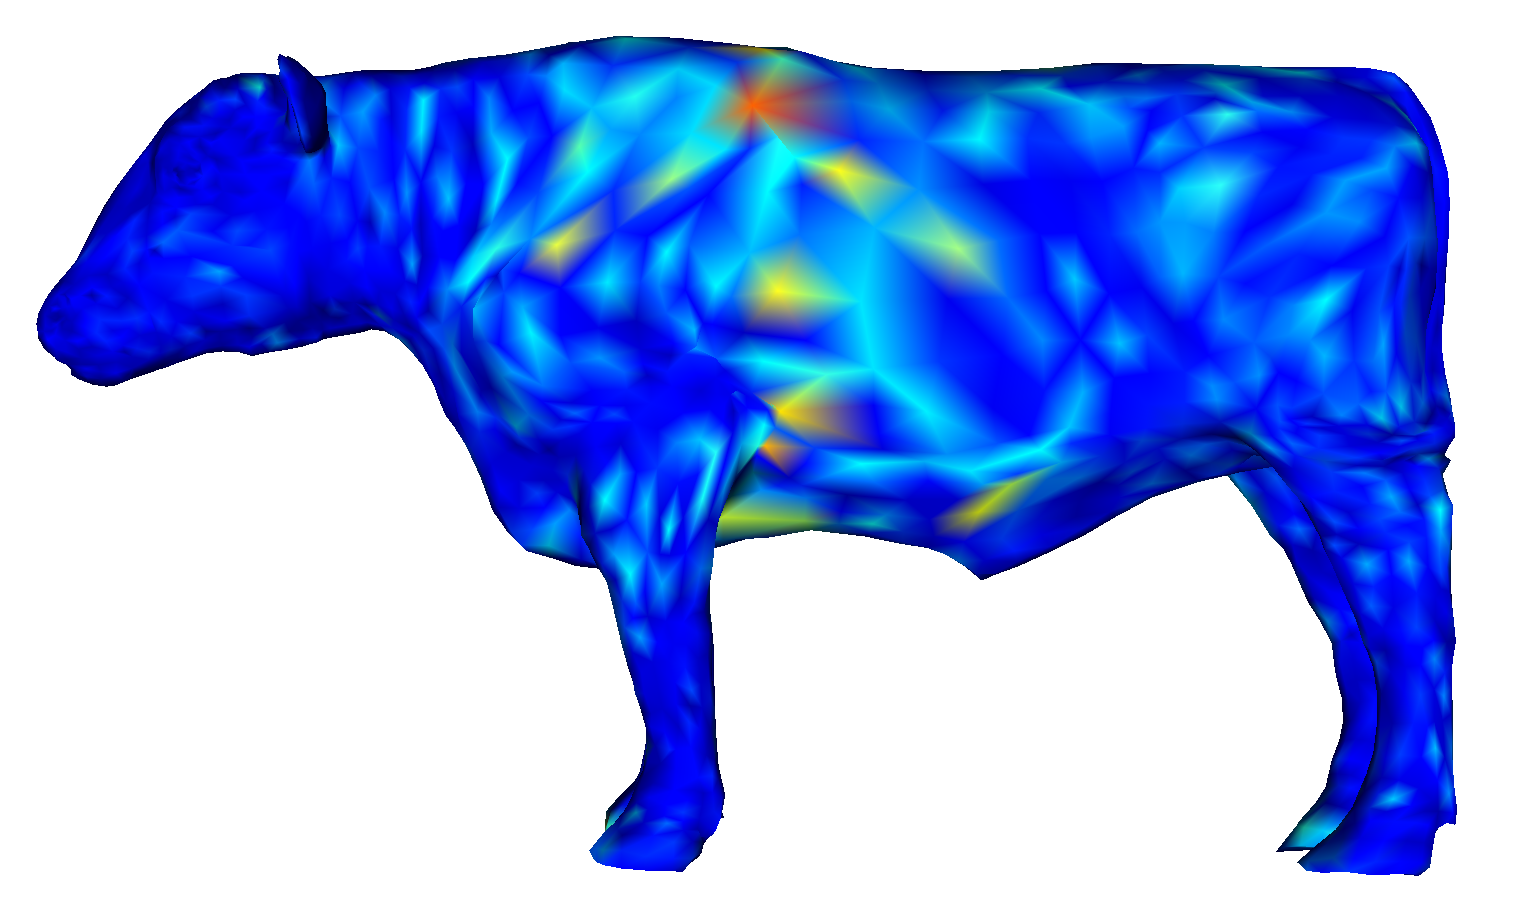
\includegraphics[width=\linewidth]{16}
        \caption{MHB, truncation}
    \end{subfigure}
    ~
    \begin{subfigure}{0.44\linewidth}
        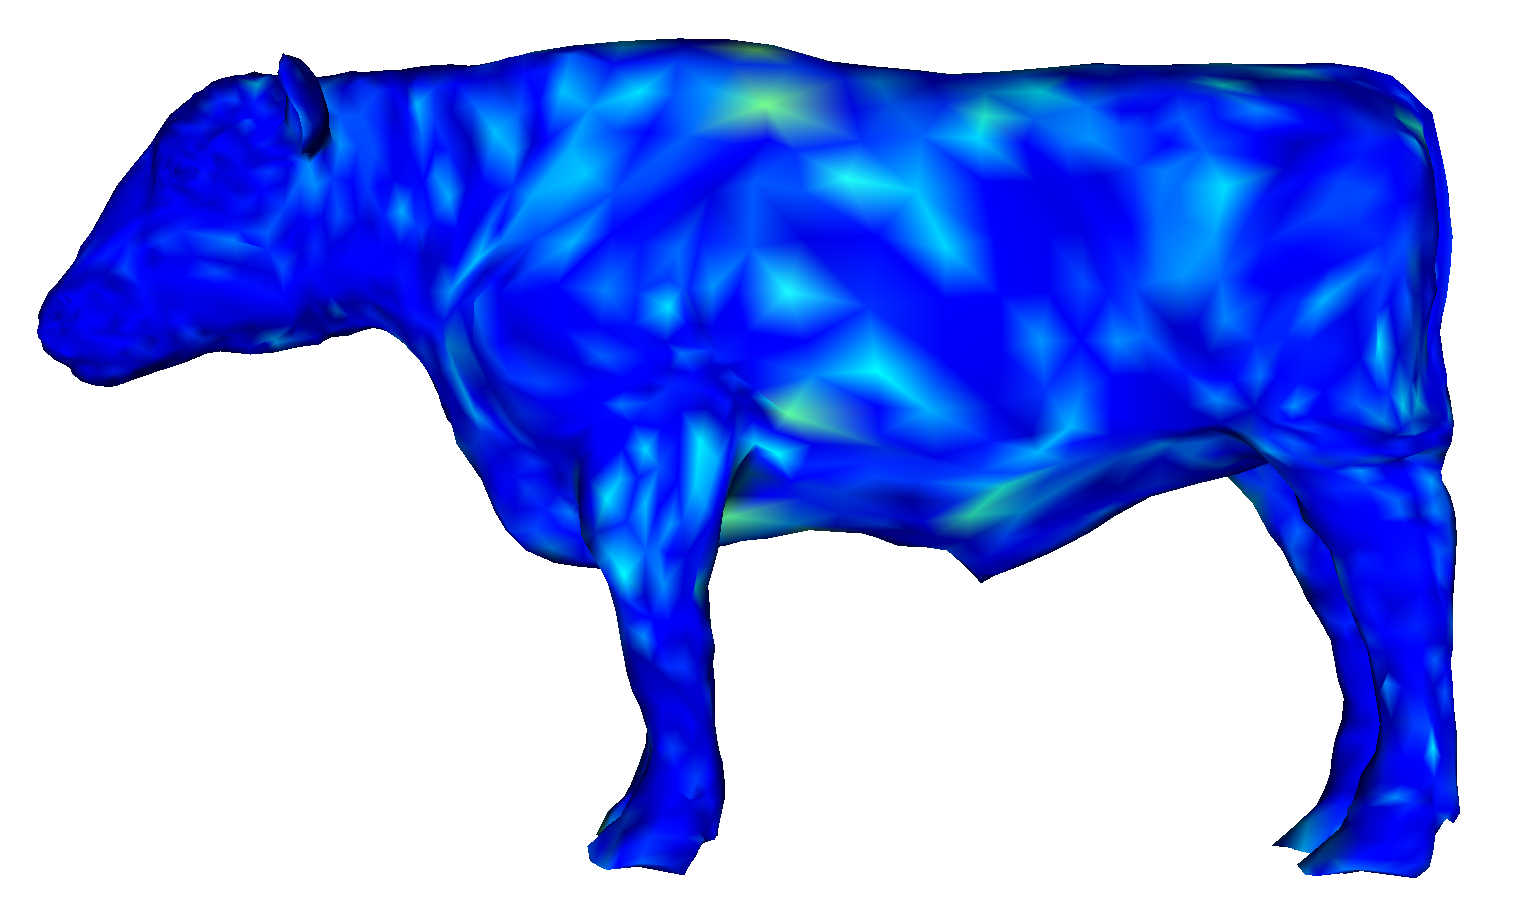
\includegraphics[width=\linewidth]{17}
        \caption{MHB, S-MP}
    \end{subfigure}
    \\
    \begin{subfigure}{0.44\linewidth}
        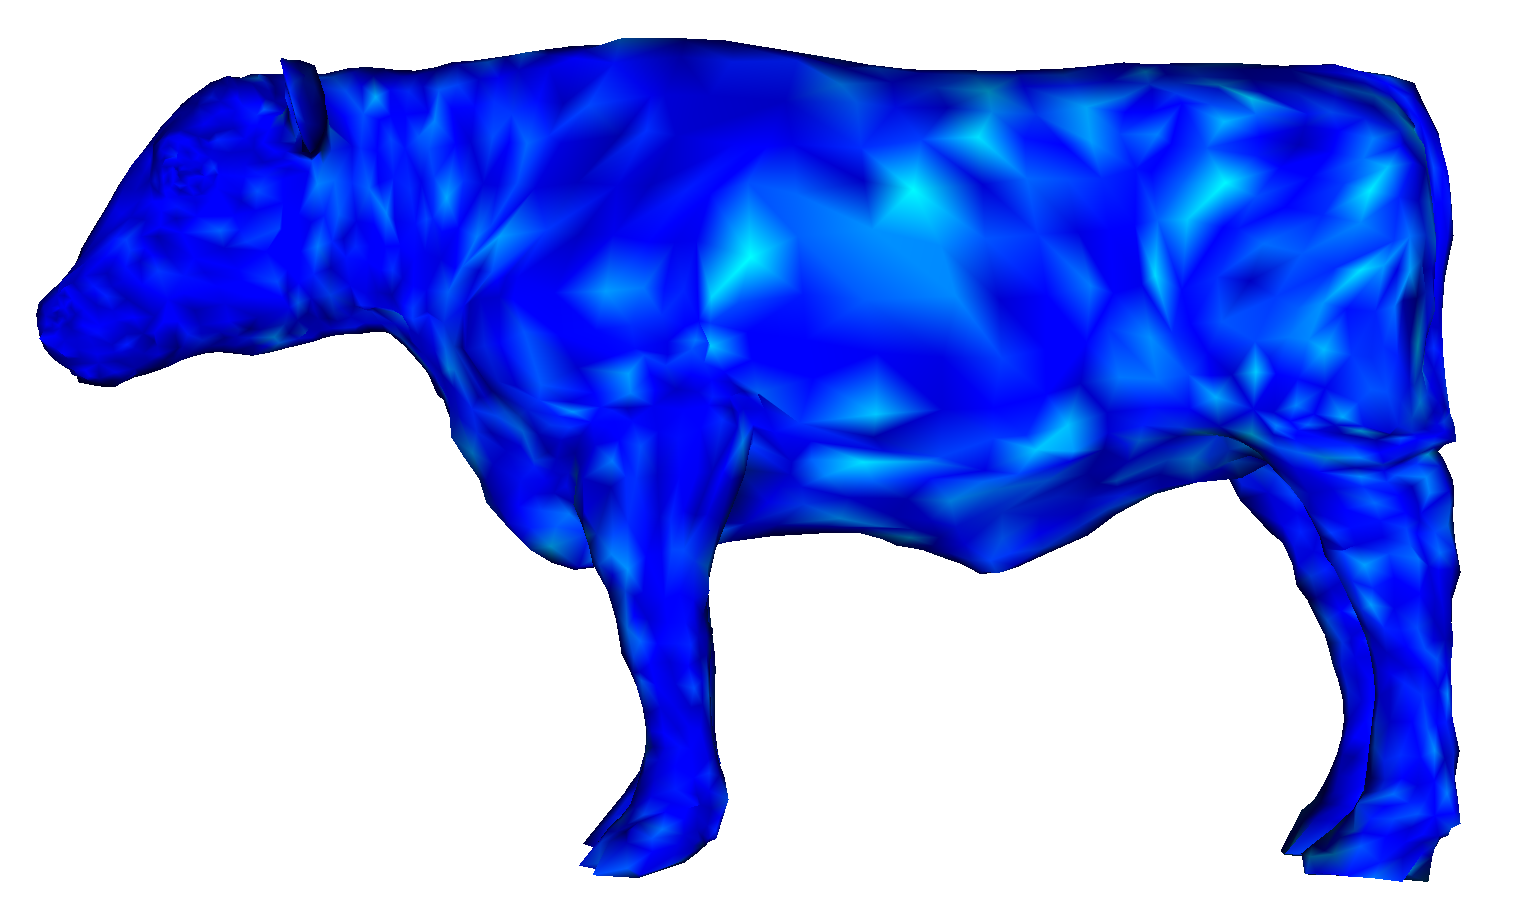
\includegraphics[width=\linewidth]{18}
        \caption{SGW, S-OMP}
    \end{subfigure}
    ~
    \begin{subfigure}{0.44\linewidth}
        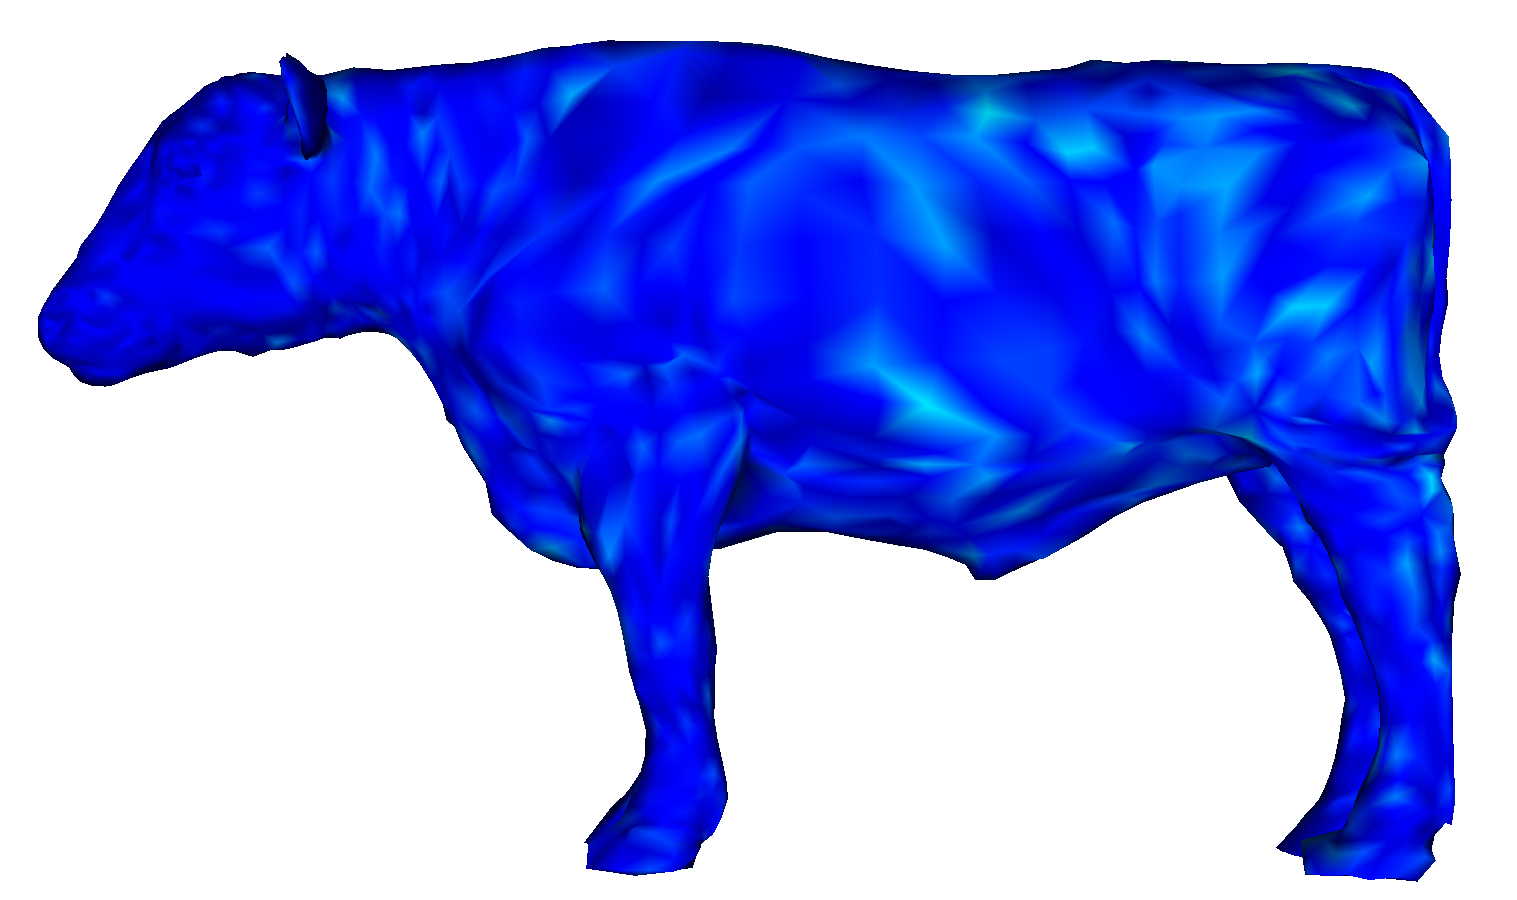
\includegraphics[width=\linewidth]{19}
        \caption{SGW+MHB, S-OMP}
    \end{subfigure}
    \\
    \begin{subfigure}{0.05\linewidth}
        (e)
    \end{subfigure}
    \begin{subfigure}{0.83\linewidth}
        \includegraphics[width=\linewidth]{20}
%        \caption{}
    \end{subfigure}
    \caption[Mesh compression performance on the cow model.]
    {Comparison of mesh compression performance
        for the cow model. (a-d) show the reconstructed meshes at 20\%
        compression ratio and visualize each vertex's positional error
        comparing with the original model. (e) shows how the
        compression errors change with the compression ratio.}
    \label{fig:coweval}
\end{figure}

\begin{figure}
    \centering
    \begin{subfigure}{0.45\linewidth}
        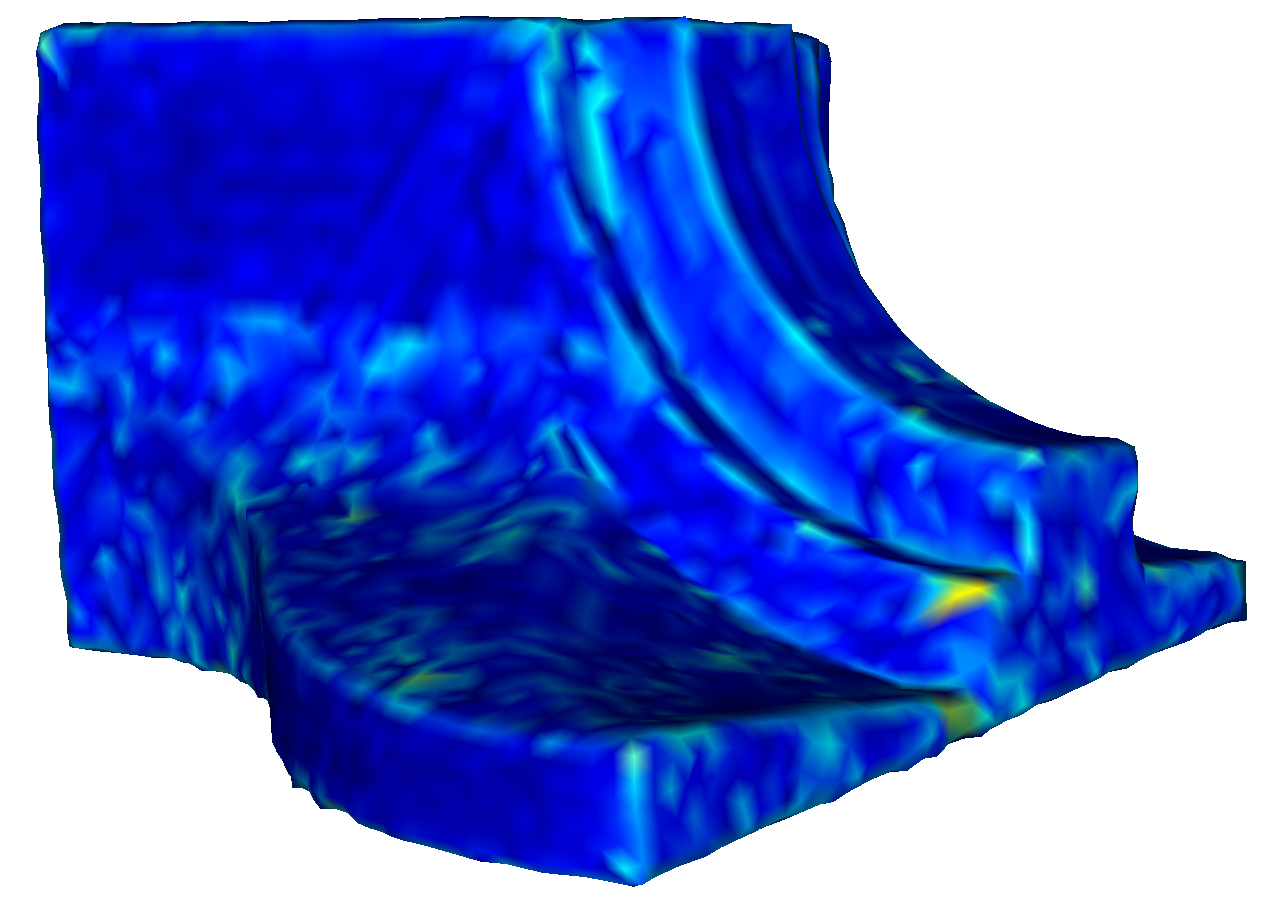
\includegraphics[width=\linewidth]{21}
        \caption{MHB, truncation}
    \end{subfigure}
    ~
    \begin{subfigure}{0.45\linewidth}
        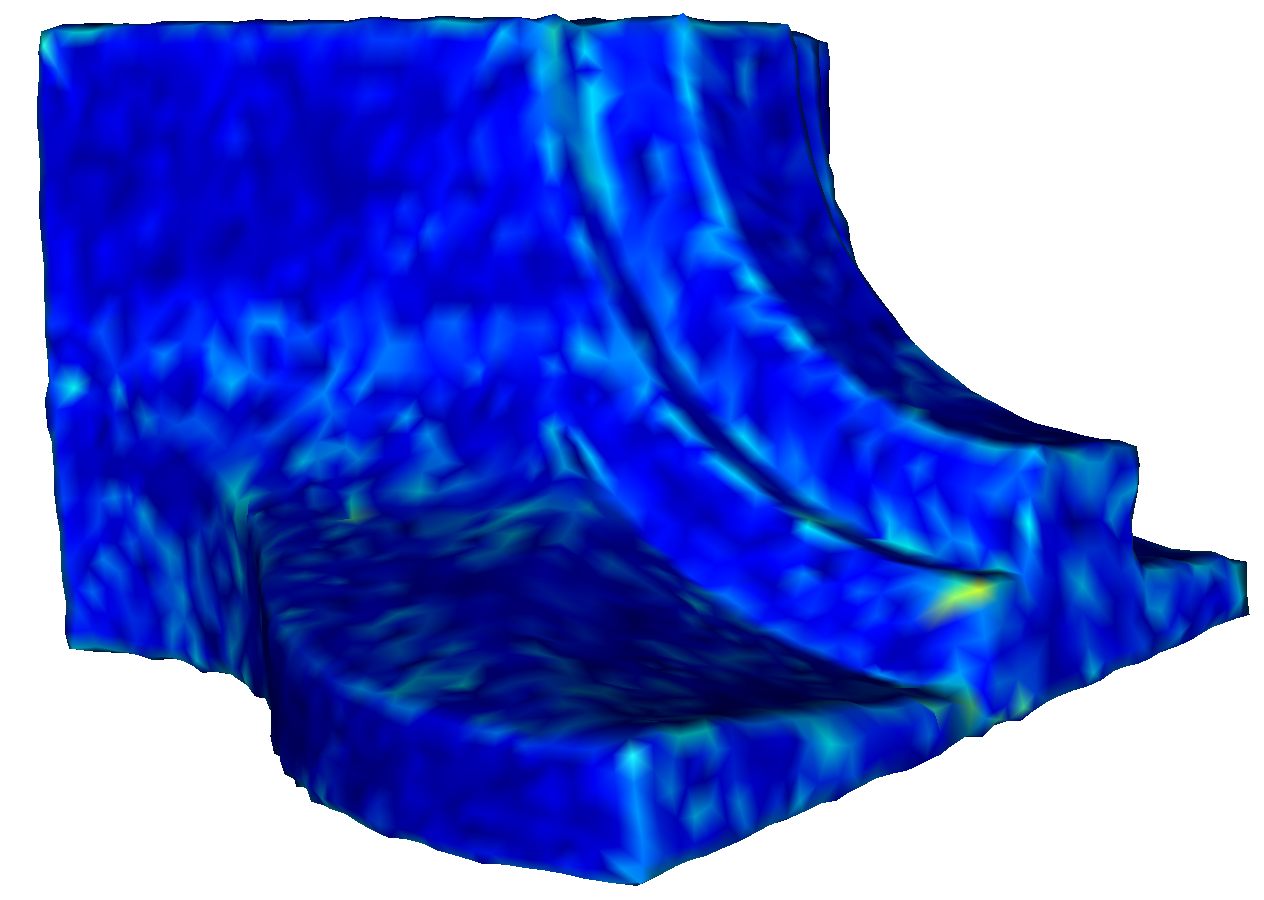
\includegraphics[width=\linewidth]{22}
        \caption{MHB, S-OMP}
    \end{subfigure}
    \\
    \begin{subfigure}{0.45\linewidth}
        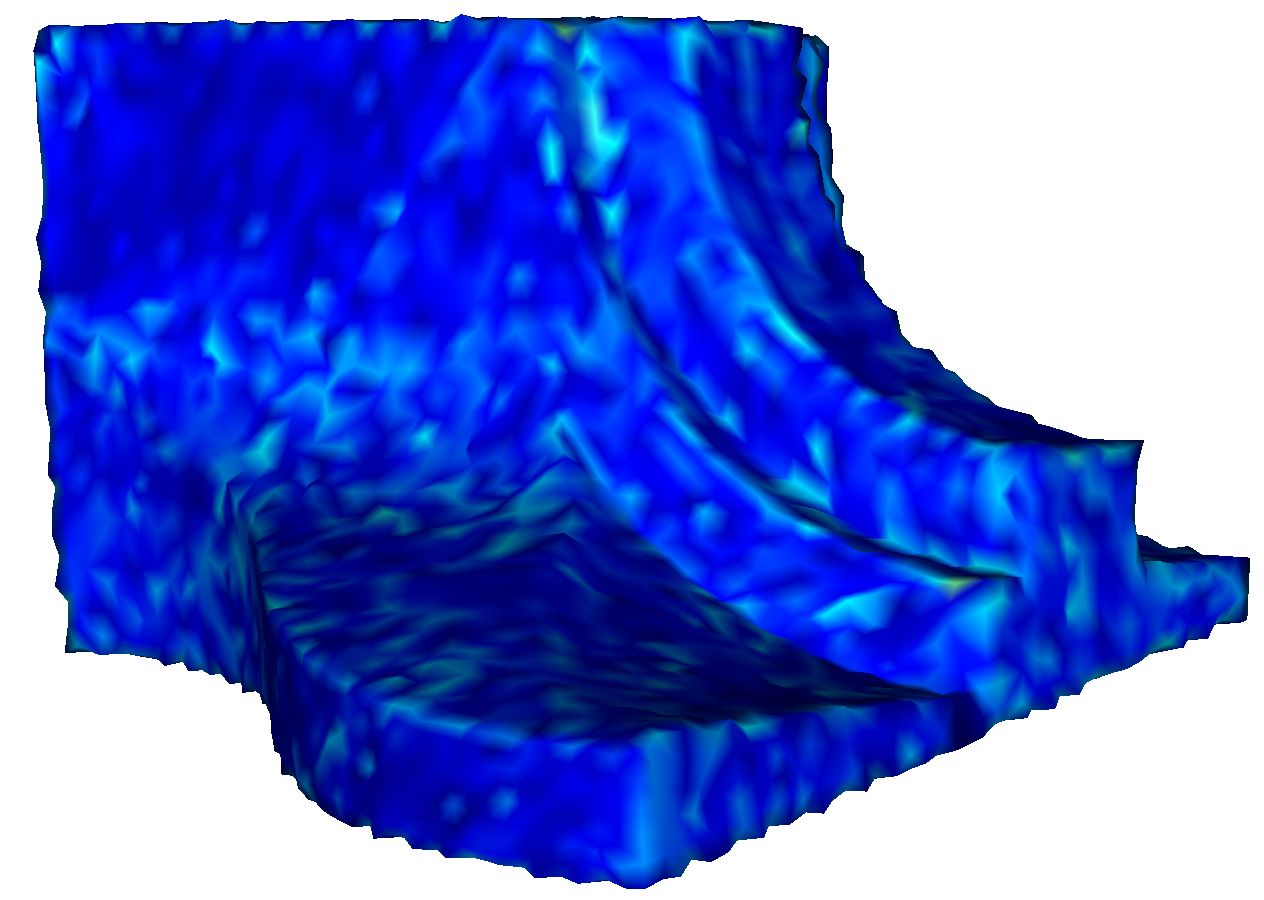
\includegraphics[width=\linewidth]{23}
        \caption{SGW, S-OMP}
    \end{subfigure}
    ~
    \begin{subfigure}{0.45\linewidth}
        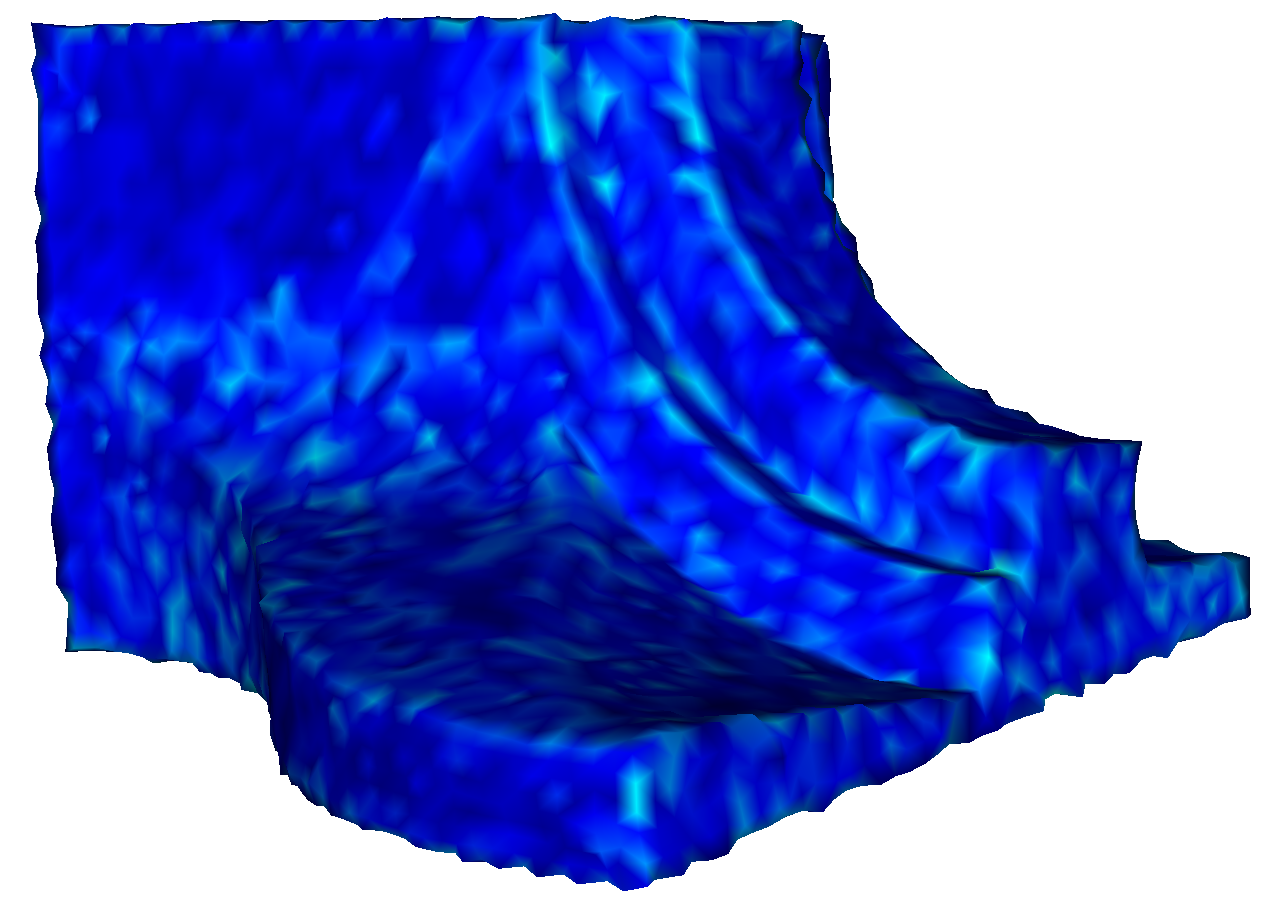
\includegraphics[width=\linewidth]{24}
        \caption{SGW+MHB, S-OMP}
    \end{subfigure}
    \\
    \begin{subfigure}{0.05\linewidth}
        (e)
    \end{subfigure}
    \begin{subfigure}{0.83\linewidth}
        \includegraphics[width=\linewidth]{25}
%        \caption{}
    \end{subfigure}
    \caption[Mesh compression performance on the fandisk model.]
    {Comparison of mesh compression performance
     for the fandisk model. (a-d) show the reconstructed meshes at
     20\% compression ratio and visualize each vertex's positional
     error comparing with the original model. (e) shows how the
     compression errors change with the compression ratio.}
    \label{fig:fandiskeval}
\end{figure}

\begin{figure}
    \centering
    \begin{subfigure}{0.45\linewidth}
        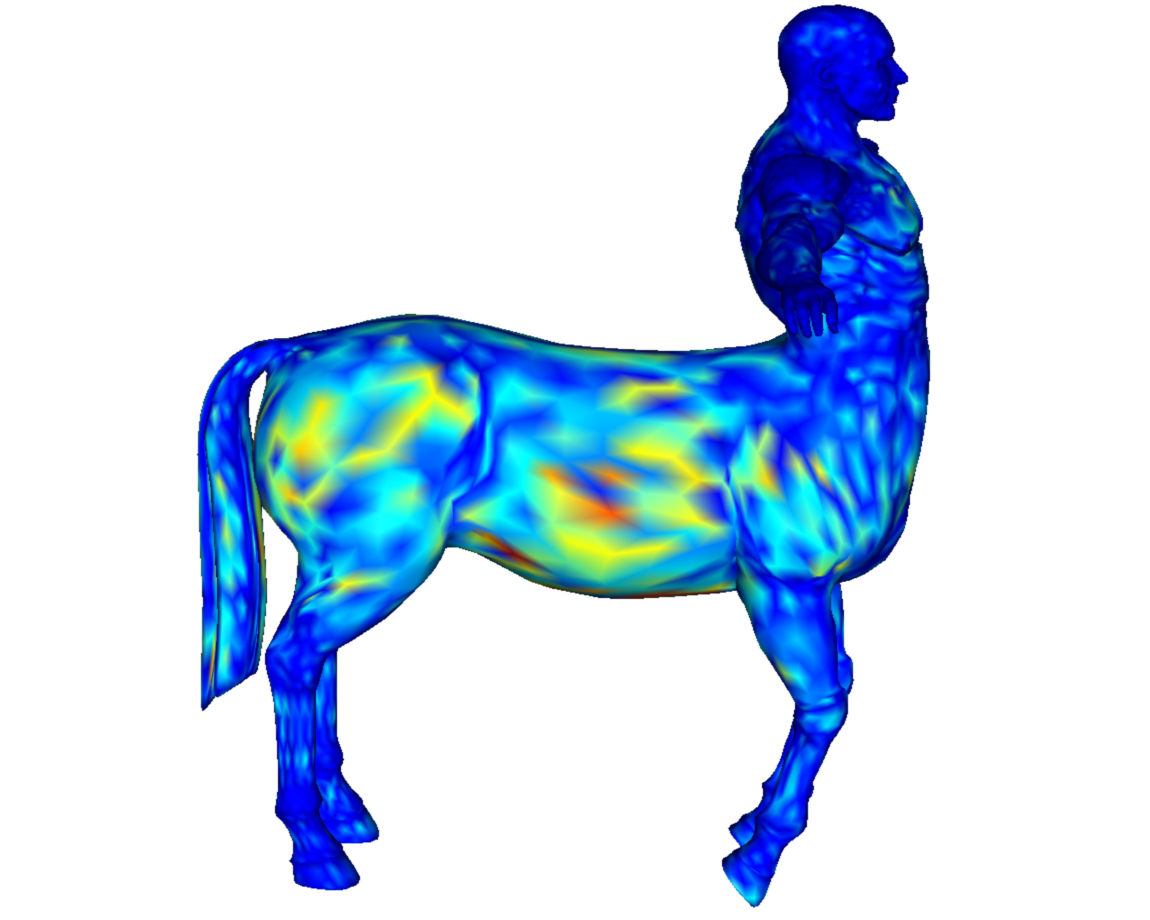
\includegraphics[width=\linewidth]{26}
        \caption{MHB, truncation}
    \end{subfigure}
    ~
    \begin{subfigure}{0.45\linewidth}
        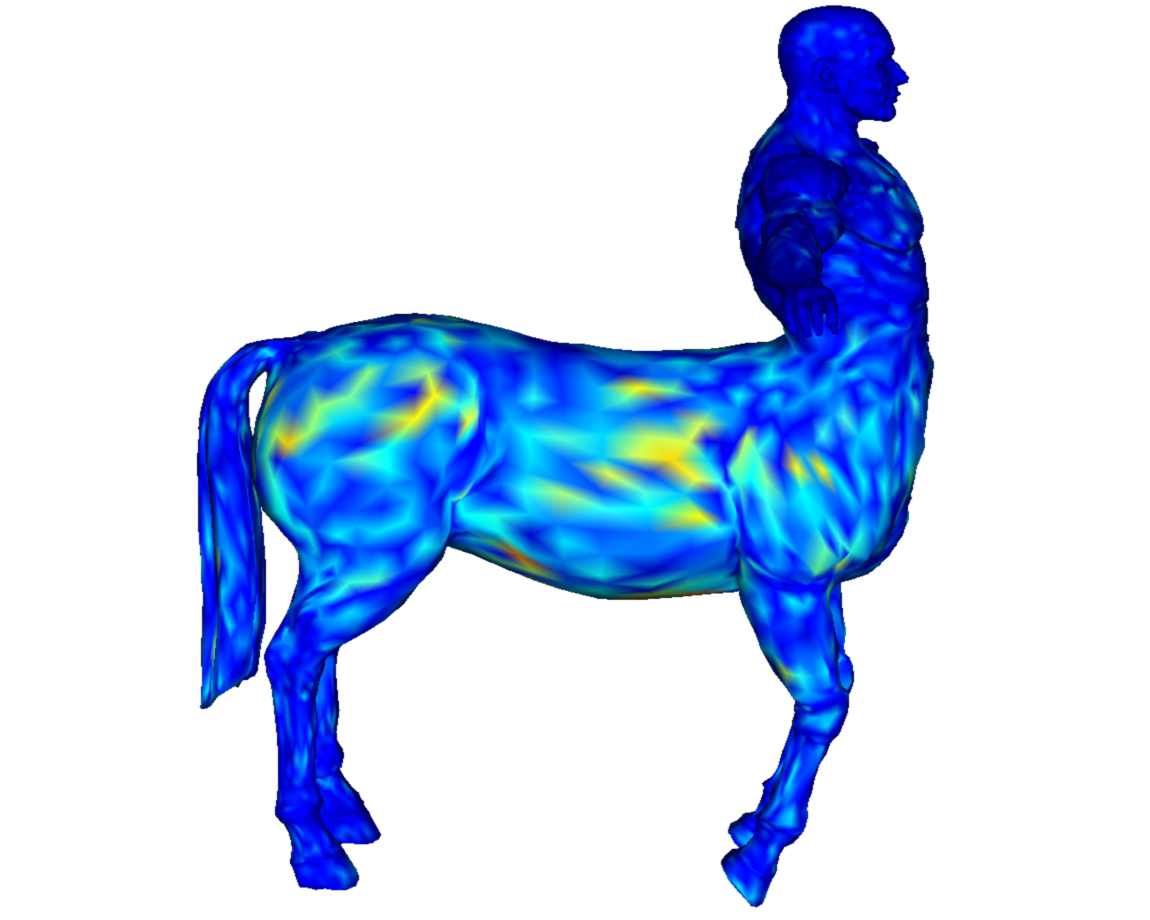
\includegraphics[width=\linewidth]{27}
        \caption{MHB, S-OMP}
    \end{subfigure}
    \\
    \begin{subfigure}{0.45\linewidth}
        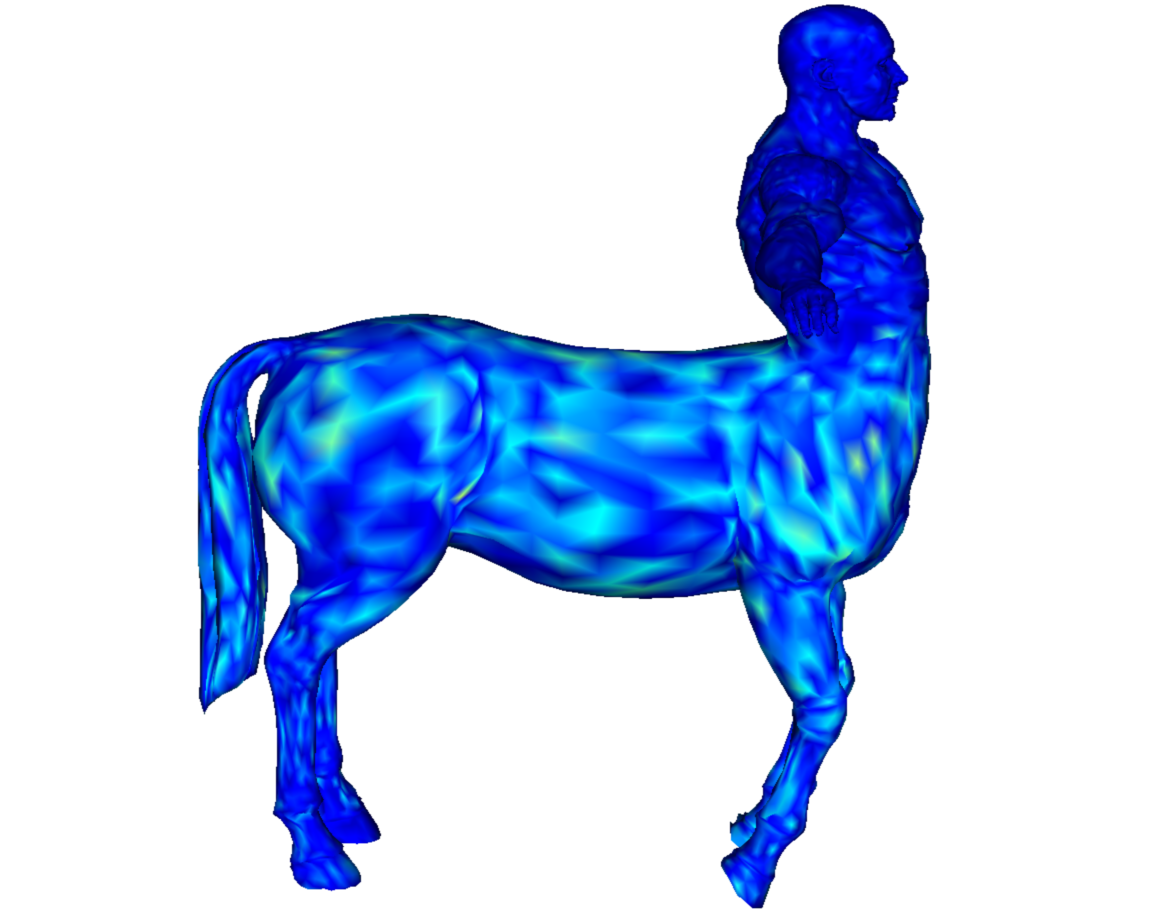
\includegraphics[width=\linewidth]{28}
        \caption{SGW, S-OMP}
    \end{subfigure}
    ~
    \begin{subfigure}{0.45\linewidth}
        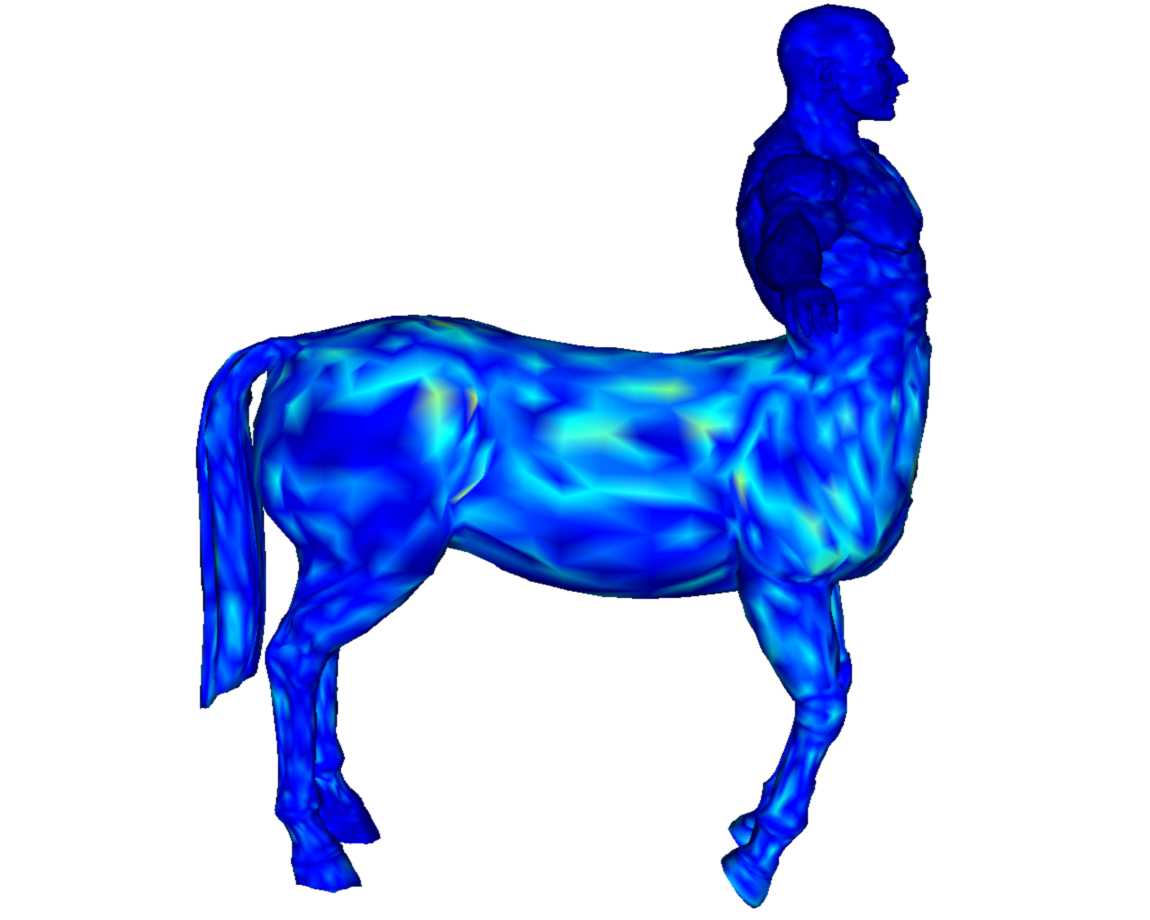
\includegraphics[width=\linewidth]{29}
        \caption{SGW+MHB, S-OMP}
    \end{subfigure}
    \\
    \begin{subfigure}{0.05\linewidth}
        (e)
    \end{subfigure}
    \begin{subfigure}{0.83\linewidth}
        \includegraphics[width=\linewidth]{30}
%        \caption{}
    \end{subfigure}
    \caption[Mesh compression performance on the centaur model.]
    {Comparison of mesh compression performance
     for the centaur model. (a-d) show the reconstructed meshes at
     20\% compression ratio and visualize each vertex's positional
     error comparing with the original model. (e) shows how the
     compression errors change with the compression ratio.}
    \label{fig:centaureval}
\end{figure}

\begin{figure}
    \centering
    \begin{subfigure}{0.44\linewidth}
        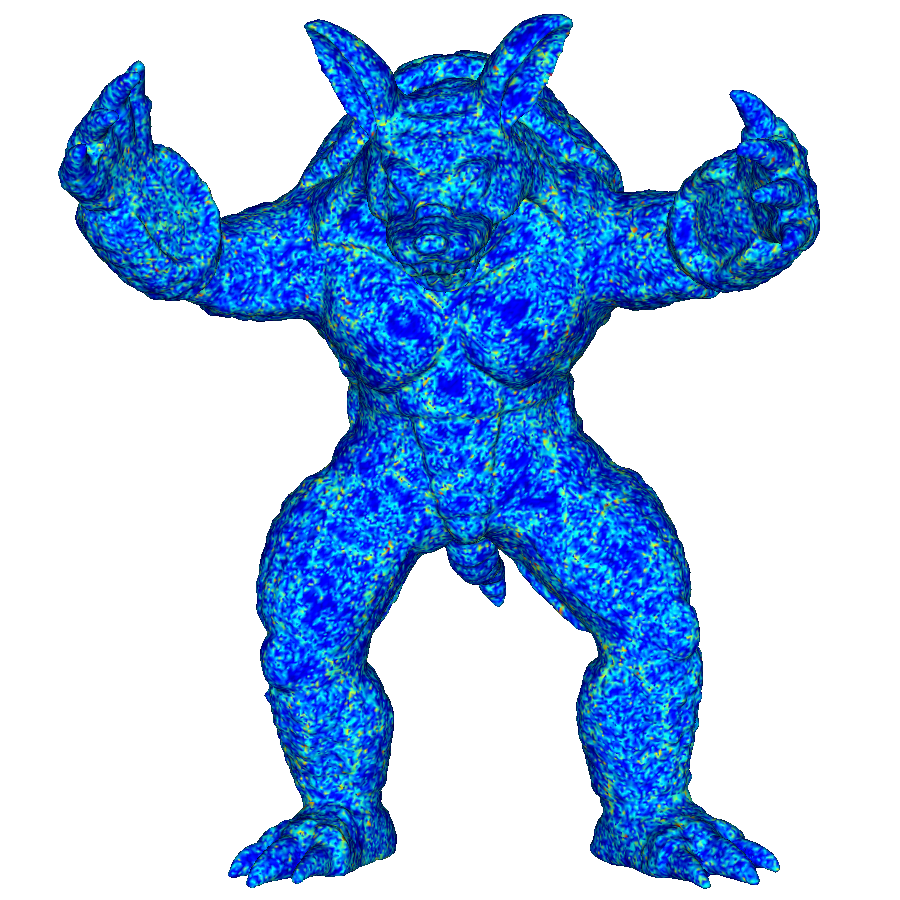
\includegraphics[width=\linewidth]{31}
        \caption{MHB, truncation}
    \end{subfigure}
    ~
    \begin{subfigure}{0.44\linewidth}
        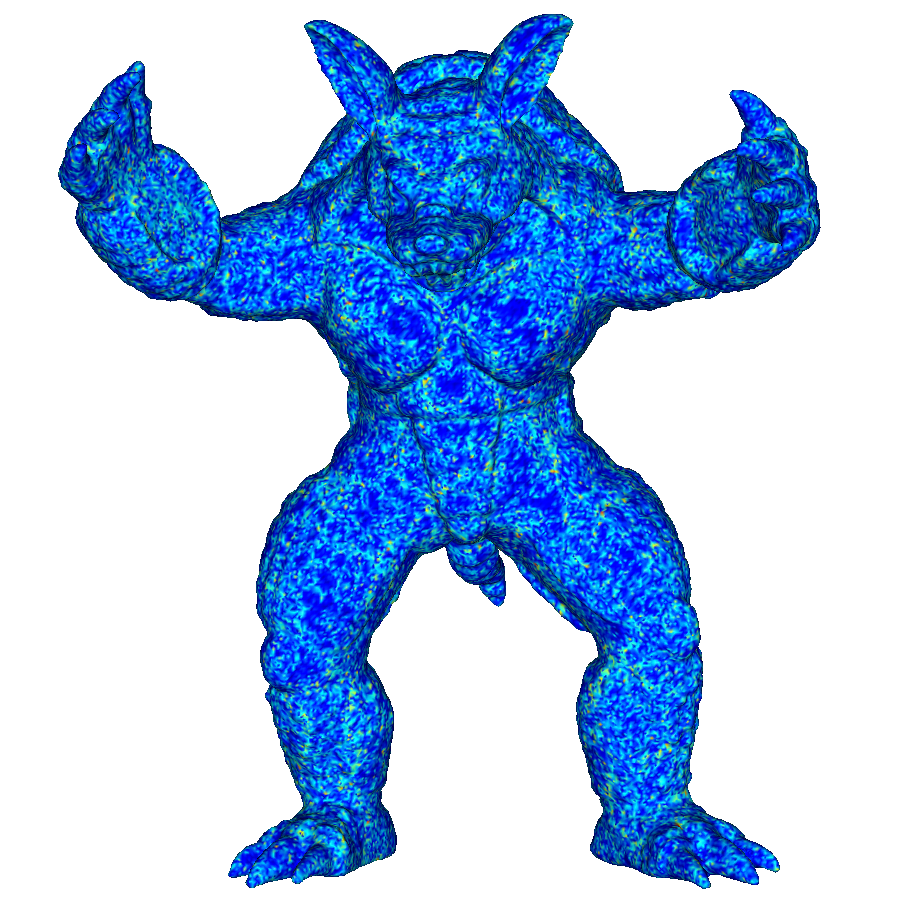
\includegraphics[width=\linewidth]{32}
        \caption{MHB, S-MP}
    \end{subfigure}
    \\
    \begin{subfigure}{0.44\linewidth}
        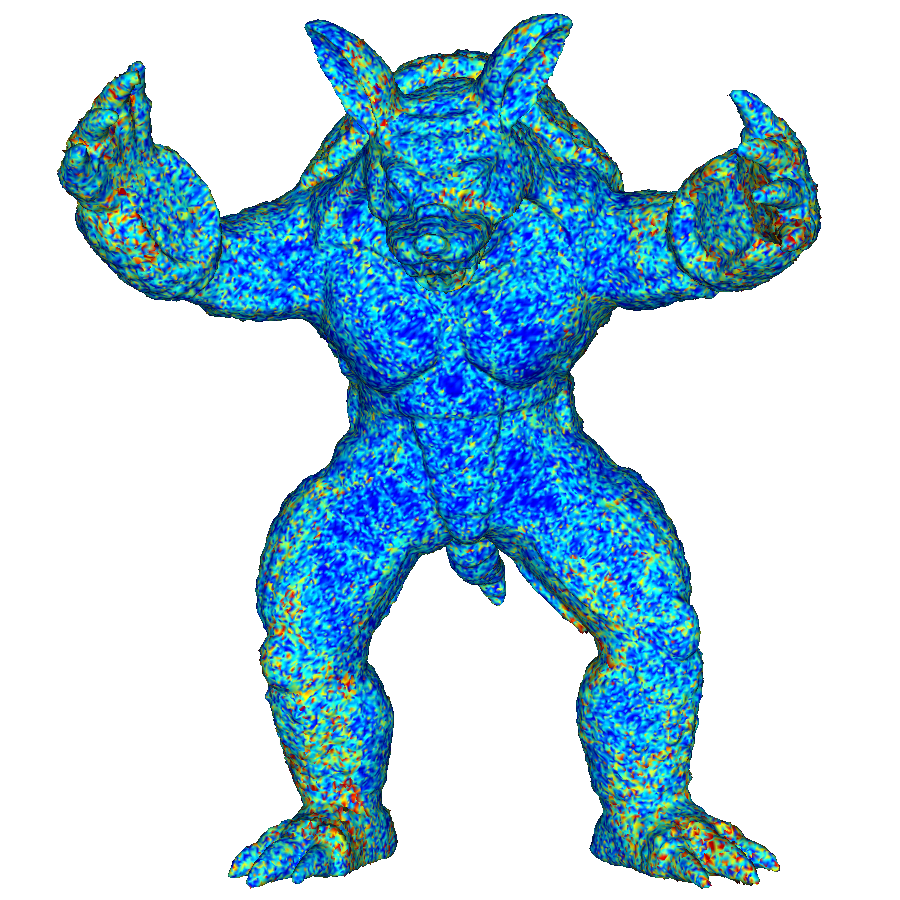
\includegraphics[width=\linewidth]{33}
        \caption{SGW, S-OMP}
    \end{subfigure}
    ~
    \begin{subfigure}{0.44\linewidth}
        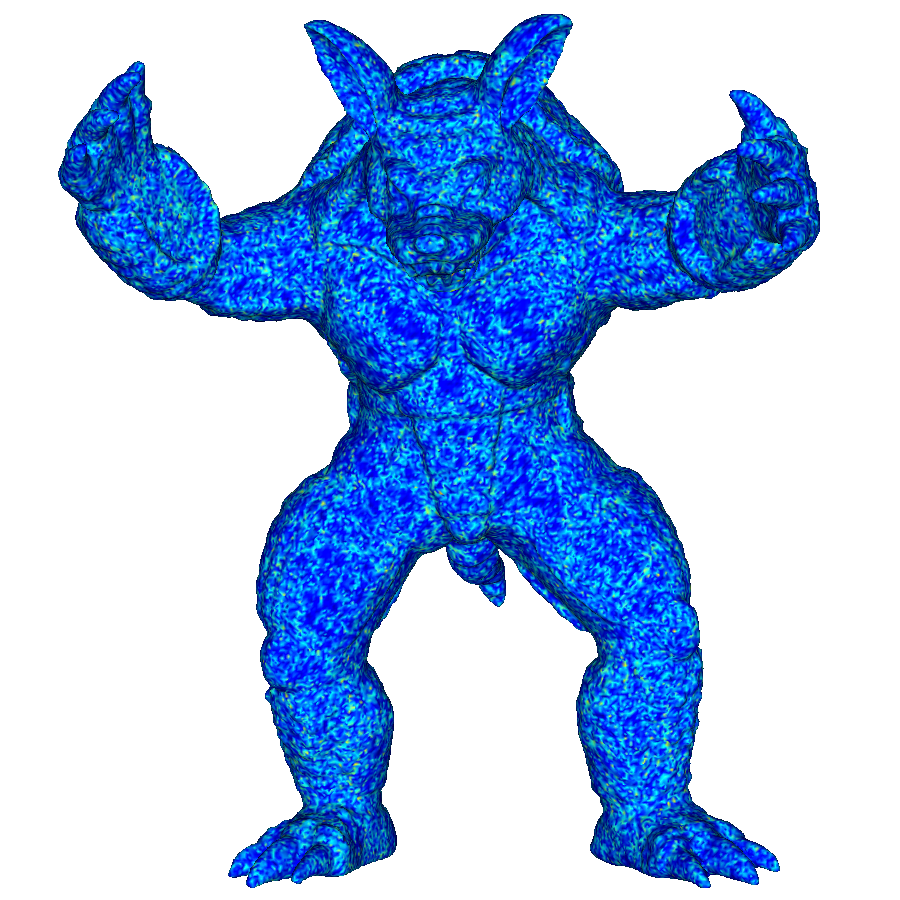
\includegraphics[width=\linewidth]{34}
        \caption{SGW+MHB, S-OMP}
    \end{subfigure}
    \\
    \begin{subfigure}{0.05\linewidth}
        (e)
    \end{subfigure}
    \begin{subfigure}{0.83\linewidth}
        \includegraphics[width=\linewidth]{35}
        %\caption{}
    \end{subfigure}
    \caption[Mesh compression performance on the armadillo model.]
    {Comparison of mesh compression performance
        for the armadillo model. (a-d) show the reconstructed meshes
        at 15\% compression ratio and visualize each vertex's
        positional error. Comparing (c) and (d), it is obvious that the SGW+MHB dictionary
        produces much smaller positional error than the SGW-only dictionary.
        (e) shows how the compression errors change with the compression
        ratio.}
    \label{fig:armadilloeval}
\end{figure}

In all our tests, we compare the compression performance between the
classical spectral compression method based on MHB coefficient
truncation \cite{Karni2000} and our sparse approximation
compression method employing three different dictionaries: (1) S-MP
with the MHB-only dictionary; (2) S-OMP with the SGW-only dictionary;
(3) S-OMP with the SGW+MHB dictionary.

\begin{table}[th]
\centering
\begin{tabular}{ |c|c|c|c|c| }
\hline
Model (\#vertices) & Ratio & Error & Error Decrease & Timing (s) \\
\hline
\multirow{2}{*}{Cow (4,315)} & 20\% & 1.91e-3 & 18.0\% & 3.4 \\
                             & 40\% & 1.12e-3 & 27.5\% & 10.5 \\
\hline
\multirow{2}{*}{Fandisk (6,475)} & 20\% & 1.09e-3 & 11.6\% & 7.2 \\
                                 & 40\% & 5.74e-4 & 28.1\% & 18.9 \\
\hline
\multirow{2}{*}{Centaur (15,768)} & 20\% & 1.03e-3 & 20.3\% & 19.6 \\
                                  & 40\% & 5.89e-3 & 37.7\% & 50.3 \\
\hline
\multirow{2}{*}{Armadillo (172,974)} & 20\% & 2.26e-3 & 9.4\% & 178.0 \\
                                     & 40\% & 1.76e-3 & 15.7\% & 354.5 \\
\hline
\end{tabular}
\caption[Statistics of compression errors and running times using different dictionary.]
{Statistics of compression errors and
    running times using the S-OMP algorithm with SGW+MHB dictionary
    (on a machine with quad-core 2.4GHz processor and 16G RAM).
    The ``Error Decrease'' column shows the decrease of compression
    error compared with the MHB truncation method.}
\label{tab:stat}
\end{table}

Fig.~\ref{fig:partitions} shows the original meshes and their
partitioning used in our experiments, including a ``cow'', a
``fandisk'', a ``centaur'', and a ``armadillo'' model. All meshes are
scaled to have unit surface area. The evaluation results are shown in
Fig.~\ref{fig:coweval}, Fig.~\ref{fig:fandiskeval},
Fig.~\ref{fig:centaureval}, and Fig.~\ref{fig:armadilloeval},
respectively. For each 3D mesh, we compute the approximation at
specified compression ratios in the ranges between 5\% and 80\%. The
overall compression quality is measured by the combined geometric and
differential error (see Eq.~(\ref{eq:metric})) w.r.t. the original
mesh. Table~\ref{tab:stat} documents the compression errors and timing
of S-OMP with SGW+MHB dictionaries, and compares the errors with the
MHB coefficient truncation method.

From the experimental results, we see that, with a properly
chosen dictionary, simultaneous sparse approximation can generate
higher-fidelity mesh compression than the MHB truncation method at the
same compression ratio. The SGW functions are a viable choice for
efficient mesh approximation, but the performance of a SGW-only
dictionary degenerates significantly when the required compression
ratio is small or the mesh is large, which is especially evident in the armadillo
model (Fig.~\ref{fig:armadilloeval}). A dictionary combining SGW and MHB
overcomes this deficiency, and its performance in mesh approximation
is consistently superior to the MHB truncation method.

\section{Chapter Summary}

In this chapter, we have developed an algorithm for sparse
approximation of 3D shapes. We employed the spectral graph wavelets to
construct the redundant dictionary of shape bases, and used
simultaneous orthogonal matching pursuit to seek a sparse
representation of the input mesh. The use of spatially-localized
wavelets makes our algorithm very suitable and powerful for better
approximating shapes with many local and fine geometric features.
Through comprehensive experiments we have demonstrated the superiority
of our algorithm for approximating complex 3D objects at different
compression ratio settings towards sparse representation.

As for the future work, we plan to investigate other
improved formulations of graph wavelets as basis vectors to enhance
the expressive power of dictionary. For example, it is potentially desirable
to have data-dependent, anisotropic wavelets that are adaptive to shape
features such as sharp corners and edges to attain more efficient and 
sparse representation of shape geometry. We also
plan to explore faster sparse approximation algorithms such as
stagewise orthogonal matching pursuit (StOMP)~\cite{Donoho2012} to
arrive at better time performance. 